\documentclass[10pt]{report}
\usepackage[utf8]{inputenc}
\usepackage[italian]{babel}
\usepackage{multicol}
\usepackage[bookmarks]{hyperref}
\usepackage[a4paper, total={18cm, 25cm}]{geometry}
\usepackage{graphicx}
\usepackage{xcolor}
\usepackage{textcomp}
\graphicspath{ {./img/} }
\usepackage{listings}
\usepackage{makecell}
\lstdefinestyle{customasm}{
  belowcaptionskip=1\baselineskip,
  frame=line,
  xleftmargin=\parindent,
  language=[x86masm]Assembler,
  basicstyle=\ttfamily,
  commentstyle=\itshape\color{purple!40!black},
}
\lstset{escapechar=@,style=customasm}
\lstnewenvironment{C}
  {\lstset{language=C++,frame=none}}
  {}
\usepackage{amssymb}
\usepackage{amsmath}
\usepackage{tikz} 
\usepackage[makeroom]{cancel}
\begin{document}
\title{Artificial Intelligence Fundamentals}
\author{Federico Matteoni}
\date{A.A. 2021/22}
\renewcommand*\contentsname{Index}
\maketitle
\begin{multicols}{2}
\tableofcontents
\end{multicols}
\pagebreak
\section{Introduction}
Prof.s: Maria Simi, Vincenzo Lomonaco\\
AI is taking over the world. Formalizing common sense is a lot more difficult. We can formalize knowledge in very specific and small domains. But is deep learning the final solution to AI? "It will transform many industries, but it's not magic. Almost all of AI's recent progress is based on one type of AI, in which some input is used to quickly generate simple response." (\textit{Andrew Ng})\\
\textit{This} AI can do supervised learning, but requires huge amount of data (tens of thousands of pictures to build a photo tagger, for example). The rule of thumb of Ng is: if a person can do a mental task with less than one second of thought, we can automate it using AI either now or in the near future.\\
The challenges are:
\begin{list}{}{}
	\item Software is not a problem, the community is open and the software can be replicated the software can be replicated
	\item Data is exceedingly difficult to get access to. Data is the defensible barrier for many businesses
	\item Talent, because downloading and applying open-source software to your data won't work. AI needs to be customized to context and data, that's why there's a war for the scarce AI talent that can do this work.
	\item Computational resources are also very important.
\end{list}
\paragraph{Deep Learning} Is only one approach inside the much wider field of ML and ML is only one approach in the wider field of AI. Book: \textit{Thinking Fast and Slow}, Kahneman. Two systems: system 1 does perceptual tasks, simple computations, system 2 instead does complex computation, recalling from memory\ldots this is a distinction in our brains.
\paragraph{Machine Learning} Is AI all about machine learning? Possible arguments against ML are:
\begin{list}{}{}
	\item Explanation and accountability: ML systems are not (yet?) able to justify in human terms their results. For some applications this is essential: knowledge must be meaningful to humans to be able to generate explanations? Some regulations requires the right to an explanation in decision-making, and seek to prevent discrimination based on race, opinions, sex\ldots (see GDPR)
	\item ML systems learn what's in the data, \textbf{without understanding what's true or false, real or imaginary, fair or unfair}. It is possible to develop unfair, bad models. People are generally more critical about information.
\end{list}
Building AI systems is a goal far from being solved, still quite challenging. Complex AI systems requires the combination of several techniques and approaches, not only ML.
\paragraph{AI Fundamentals} Is mostly about reasoning and \textit{slow thinking}. Different approaches, "good old-fashioned artificial intelligence" or "symbolic AI": teaching about the foundations of the discipline, now 60 years old.
\paragraph{Symbolic AI} High-level human readable representations of problems, the general paradigm of searching for a solution, knowledge representation and reasoning, planning. Dominant paradigm from the mid 1950s until late 1980s.\\
Central to the building of AI systems is the physical symbol systems hypothesis (PSSH), formulated by Newell and Simon (\textit{Computer Science as Empirical Inquiry: Symbols and Search})\\
The approach is based on the assumption that many aspects of intelligence can be achieved by the manipulation of symbols (the PSSH): \textit{a physical symbol system has the necessary and sufficient means for general intelligent action}.\\
Human thinking is a king of symbol manipulation system (so a symbol system is \textbf{necessary} for intelligence), and machine can be intelligent (a symbol system is \textbf{sufficient} for intelligence). This cannot be prove, we can only collect empirical evidence: observation and experiments on human behavior in tasks requiring intelligence, and solving tasks of increasing complexity.
\paragraph{Strong and Weak AI} The Chinese room argument, by John Searle, introduced the following distinction: strong ai relies on the \textit{strong} assumption that human intelligence can be reproduced in all its aspects (general AI), including adaptivity, learning, consciousness\ldots, while weak AI is the simulation of human-like behavior, without effetctive thinking or understanding, no claim that it works like the human mind. Dominant approach today, fragmented AI.\\
One strong argument against strong AI is the lack of needs by the systems: biological need, safety, relationships, self esteem, self-actualization (Maslow's hierarchy of needs).\\
\textit{What stands in the way of all-powerful AI is not a lack of smarts: it's that computers can't have needs, cravings or desires.}\\\\
\textbf{AI is the enterprise of building intelligent computational agents}
\paragraph{Agents} An agent is something that acts in an environment. We are interested in what an agetn does, that is how it acts. We judge and agent by its action. An agent acts intelligently when: what it does is appropriate given the circumnstances and its goals, it is flexible to changing envoronments and changing goals, learns from experience, makes appropriate choices given its perceptual and computational limitations.\\
\textbf{Computational agent} is an agent whose decsiions about its actions can be explained in terms of computation and implkemented on a physical device.
\begin{list}{}{}
	\item \textbf{Scientific Goal}: undestrand the principles that make intelligent behavior possibile in natural or artificial systems
	\item \textbf{Engineering Goal}: design and synthesis of userful, intelligente artifacts, agents that are useful in many applications
\end{list}
%TODO lista slide 5
\paragraph{Artificial Intelligence} Artificial intelligent is not the opposit of real intelligence. Intelligence cannot be \textit{fake}: in an artificial agent behaves intelligently, it is intelligent. It is only the external behavior that defines intelligence, according to the \textbf{Turing Test} (weak AI). So \textbf{artificial intelligence is real intelligence created artificially}.\\
More updated test: Winograd schemas.\\
\textbf{Human intelligence}: biology (surviving various habitats), culture (language, tools, concepts, wisdom passed from parents and teachers to children) and life-long learning experience (learning throughout life). Another form is social intelligence, exhibited by communities and organizations.\\\\
So agents are situated in environments, inputs are abilities, goals, prior knowledge, stimuli and past experiences, and outputs actions which affect the environment.
\begin{center}
	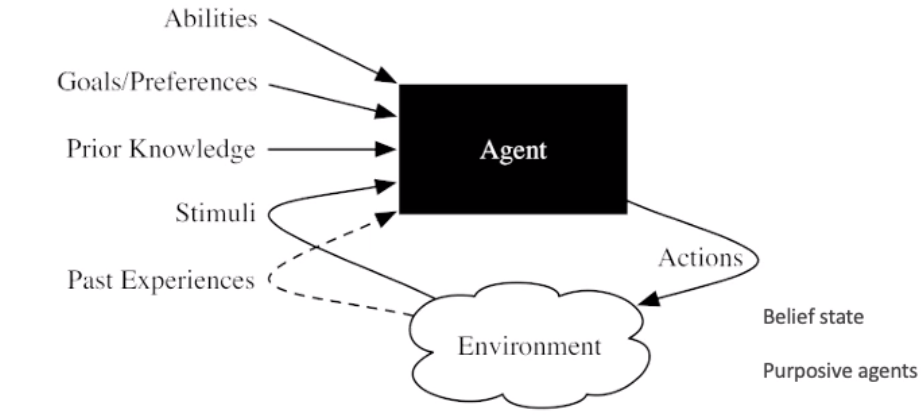
\includegraphics[scale=0.5]{1.png}
\end{center}
\paragraph{Design process}
\begin{list}{}{}
	\item design time computation, that goes into the design
	\item offline computation, that the agent can do before acting in the world (ex: specializing the model)
	\item online computation, done by the agent that is acting
\end{list}
Designing an intelligent agent that can adapt to complex environments and changing goals is a major challenge. Two strategies: simplify environments and build strong reasoning systems for these simple environments, or build simple agents for natural/complex environments simplifying the task.\\
\textbf{Steps} in the design process:
\begin{list}{}{}
	\item define the task in natural language, what need to be computed
	\item define what is a solution and its quality: optimal, satisfying, aproximately optimal, probable\ldots
	\item formal representation for the task, choosing how to represent knowledge for the task, including representations suitable for learning.
	\item compute an output
	\item interpret output as solution
\end{list}
\begin{center}
	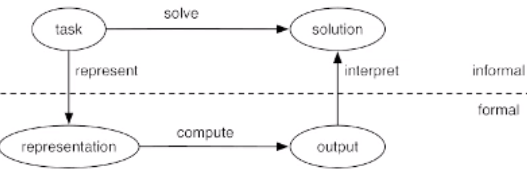
\includegraphics[scale=0.5]{2.png}
\end{center}
\paragraph{Levels of abstraction} A model of the world is a syumbolic rtepresentation of the beliefs of the agents. In is necessarily an abstraction: more abstract representations are simpler and human-readable but they may not be effective enough. Low level descriptions are more detailed and accurate but more complex too. Multiple level of abstractions are possibile (hierchical design). Two levels always present in the design: knowledge level (what the agent knows and its goals, not in terms of how we represent) and the symbol level (internal representation and reasoning system). \textbf{Modularity} extent to which a system/task can be decomposed \begin{list}{}{}
	\item flat: not modular
	\item modular: interacting modules that can be understood on their own
	\item hierarchical: modules are decomposed into simpler modules
\end{list}
\textbf{Planning horizon} how far ahead in time the agent plans \begin{list}{}{}
	\item non planning agent
	\item finite horizon planner: looks for a fixed amount of stages, greedy if only one step ahead
	\item indefinite horizon planner: finite but not predetermined number of stages
	\item infinite horizon planner: keeps planning forever (ex: stabilization module of a legged robot)
\end{list}
\textbf{Representation} concerns how the state of the world is described \begin{list}{}{}
	\item Atomic states
	\item feature-based representation: set of propositions that are true or false (PROP, CSP, most ML)
	\item individuals and relations, or relational representation
\end{list}
\textbf{Computational limits} that determines whether an agent has \begin{list}{}{}
	\item perfect rationality, reasons about the best actions without constraints
	\item bounded rationality, decides on the best action that it can find given its limits
\end{list}
An anytime algorithm is an algorithm where the solution improves with time.\\
\textbf{Learning dimensions} determines whether \begin{list}{}{}
	\item knowledge is given in advance, or
	\item knowledge is learned (from data or past experience)
\end{list}
Learning typically means finding the best model th %TODO
\textbf{Uncertainty}, which can be \begin{list}{}{}
	\item in sensing (fully/partially observable states)
	\item about the effects of the actions (deterministic/stochastic)
\end{list}
\textbf{Preference} dimension which considers thetehr the agent has
\begin{list}{}{}
	\item goal (achievemtn goal a proposition true in a final state, or mainentance goal, proposition true in all psobbile states)
	\item complex preferences, involving trade-offs among the desiderability of various\ldots %TODO
\end{list}
\textbf{Number of agents}\begin{list}{}{}
	\item single agent reasoning
	\item multi agent resoning
\end{list}
\textbf{Interaction} considers wheter the agent does:
\begin{list}{}{}
	\item offline reasoning or
	\item online reasoning
\end{list}
\paragraph{Agent Architectures} Agent interacts with an environment, receives informations with sensors and acts in the world with actuators. Robot: physical body. Program: software agent, digital environment.\\
Agent is made of body and controller, which receives percepts from the body and sends command to the body. A body includes sensors that converts stimuli into percepts and actautors that convert commands into actions.
\begin{center}
	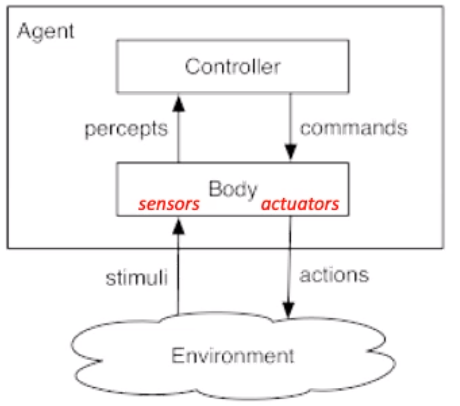
\includegraphics[scale=0.5]{3.png}
\end{center}
Bot sensors and %TODO
Agents act in time. $T$ is a set of time points, with start at 0, totally ordered, discrete and each $t$ has a next time $t+1$.\\
Percept trace/stream: function of time into percepts (past, present, future)\\
Command trace: a function of time into commands (past, present, future)\\
History at time $t$: percepts up to $t$ and commands up to $t-1$
\paragraph{Causal Trasduction} Function from history to commands. Transduction comes from \textit{finite state transducers}, where both new states and commands are emitted. "Causal" because only previous and current percepts and previous commands can be considered. A controller ideally implements a causal transduction.\\
But complete history is usually unavailable, only the memory of it. The belief state of an agent at time $t$ is all the information that the agent remembers from the previous times. The behavior of an agent can be described by two functions:
\begin{list}{}{}
	\item \textbf{Belief State function} $\textsl{remember}:S\times P\rightarrow S$ with $S$ being the set of belief states and $P$ the set of percepts
	\item \textbf{Command function} $\textsl{command}:S\times P \rightarrow C$ with $C$ being the set of commands.
\end{list}
The controller implements both, an approximation of the causal transduction.
\paragraph{Problem Solving as search} The dominant approach to AI is formulating a task as a search in a state space. The paradigm is as follows:
\begin{list}{}{}
	\item Define a goal (a set of states, a boolean test function\ldots)
	\item Formulate the task as a search problem: define a representation for states and define legal actions and transition functions
	\item Find a solution (a sequence of actions) by means of a search process
	\item Execute the plan
\end{list}
This is a basic technique in AI: search happens inside the agent, it's the planning stage before acting. It's different from searching the world, when an agent may have to act in the world and interleave an action with planning.\\
Search is a general paradigm, underlying much of the artificial intelligence field. An agent is usually given only a description of what it should achieve, not an algorithm to solve it. The only possibility is to search for a solution. Searching can be computationally very hard (NP-Complete).\\
Humans are able to solve specific instances by using their knowledge about the problem. This extra knowledge is called \textbf{heuristic knowledge}.
\paragraph{Assumptions in classic problem solving} Problem solving agents are goal driven agents, that work under simplified assumptions made in the design process.
\begin{list}{}{}
	\item States are treated as black boxes: we only need to know the heuristic value and whether they are a goal by applying the boolean goal function. The internal structure doesn't matter from the point of view of search algorithms. \textbf{Atomic representations}.
	\item The agent has \textbf{perfect knowledge} of the state (full accessibility), no uncertainty in sensors.
	\item Actions are \textbf{deterministic}, so that the agent know the consequences of its actions.
\end{list}
The state space is generated incrementally: can be infinite, so may not fit in memory.
\paragraph{Problem formulation} A problem is defined formally by five components:
\begin{list}{}{}
	\item \textbf{Initial state}
	\item \textbf{Possible actions} in state $s$, $\textsl{Actions}(s)$
	\item \textbf{Transition model}: a function $\textsl{Result}: \textsl{State}\times\textsl{Action}\rightarrow \textsl{State}$\\
	$\textsl{Result}(s,a) = s'$, a \textbf{successor state}
	\item \textbf{Goal states} are defined by a boolean function\\
	$\textsl{Goal-Test}(s) \rightarrow\{\textsl{true}, \textsl{false}\}$
	\item $\textsl{Path-cost}$ function, that assigns a numeric cost to each path. The sum of the cost of the actions on the path $c(s, a, s')$
\end{list}
\paragraph{Graphs for searching} A (directed) graph consists of a set $N$ of nodes and a set $A$ of arcs, which are ordered pairs of nodes. Node $n_2$ is a neighbor/successor of $n_1$ if $\exists\:(n_1, n_2)\in A$, and a path is a sequence of nodes $(n_0,\ldots,n_k)$ such that $(n_{i-1}, n_i)\in A$ with length $k$.\\The cost of the path is the sum of the costs of its arcs $\textsl{cost}((n_0,\ldots,n_k)) = \sum_{i=1}^k \textsl{cost}((n_{i-1}, n_i))$.\\
A \textbf{solution} is a path from a start node to a goal node and an \textbf{optimal solution} is one with minimum cost.
\paragraph{Search algorithms} A problem is given as input to a search algorithm. A solution to a problem is a path (actions sequence) that leads from the initial state to a goal state.\\
\textbf{Solution quality} is measured by the path cost function and an optimal solution has the lowest path cost among all solutions. Different strategies (algorithms) for searching the state space may be characterized by:
\begin{list}{}{}
	\item Their time and space complexity, completeness, optimality\ldots
	\item Uninformed search methods vs informed/heuristic search methods, which use an heuristic evaluation function of the nodes
	\item Direction of search (forward or backwards)
	\item Global vs local search methods
\end{list}
\subparagraph{Generic search algorithm}
\begin{verbatim}
	input:
		a graph
		a set of nodes
		boolean function goal(n) that tests if n is a goal node
	
	frontier := {s | s is a start node}
	while frontier is not empty:
		select and remove path (n0, ..., nk) from frontier
		if goal(nk):
			return (n0, ..., nk)
		for each neighbor n of nk
			add (n0, ..., nk, n) to frontier
	end while
	return fail
\end{verbatim}
\subparagraph{Other algorithms} With $b$ max number of successors, $d$ depth of solution and $m$ max distance of solution. \begin{list}{}{}
	\item \textbf{Breadth and Depth search} Respectively:
		\begin{center}
			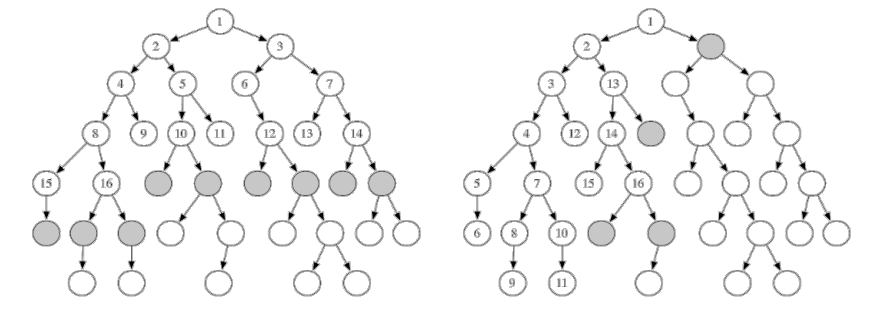
\includegraphics[scale=0.75]{4.png}
		\end{center}
		\textbf{Breadth search}: complete, optimal, time $O(b^d)$, space $O(b^d)$\\
		\textbf{Depth search}: not complete, time $O(b^m)$, space $O(bm)$
	\item \textbf{Depth bounded search}: supposes to know the distance of the solution, performs depth-first up to a limit without giving up completeness
	\item \textbf{Iterative deepening}: tries depth limit 1, then 2, then 3 and so on, freeing memory from one iteration to the next.
	\item \textbf{Uniform cost search}: at each stage, selects a path on the frontier with lowest cost.\\
	The frontier is priority queue ordered by path cost, so the first path to goal is the least-cost path. When arc costs are equal is equivalent to breadth-first search.\\
	This strategy is complete, provided that the branching factor is finite and there is some $\epsilon > 0$ such that all the costs are $> \epsilon$. It's also optimal, since it guarantees that the paths with lower costs are found first.
\end{list}
\subparagraph{Heuristic search} The idea is to not ignoring the goal when selecting the paths. Often there's extra knowledge that can be used to guide the search: \textbf{heuristics}, provided by an heuristic function $h:N\rightarrow R \Rightarrow h(n)$ is the estimate of the cost of the shortest path from node $n$ to the goal node.\\
$h$ needs to be efficiently to compute. An \textbf{admissible heuristic} $h^*(n)$ is a non-negative heuristic function that \textbf{under-estimates} the minimum cost of a path from a node $n$ to a goal: $\forall\:n\:\:\:h(n) \leq h^*(n)$\\\\
\textbf{Best first search} selects the most promising node on the frontier according to the heuristic function.
\subparagraph{$A^*$ search} With an heuristic function in the form $f(n) = g(n) + h(n)$ with:
\begin{list}{}{}
	\item $g(n)$ being the cost of path leading to $n$ (so the previous path up until $n$, $\textsl{cost}(n)$)
	\item $h(n)$ is an admissible heuristic (so, $h(n) \geq 0$)
\end{list}
Then $f(n)$ estimates the total path cost of going from a start node to a goal via $n$. The special cases are $h = 0$ (lowest cost search) and $g = 0$ (greedy best first).\\
Properties of $A^*$:\begin{list}{}{}
	\item Complete
	\item Always finds an optimal solution, if the branching factor is finite and arc costs are bounded above 0 (which means that $\exists\:\epsilon > 0\:|$ arc costs are $> \epsilon$)
	\item Optimiziations are possibile when searching graphs
	\item The operate some sort of graph pruning:
	\begin{list}{}{}
		\item \textbf{Cycle pruning}: doesn't add nodes to the frontier with states already encountered along the path (easy)
		\item \textbf{Multiple-path pruning}: maintains an explored set of nodes that are at the end of paths that have been expanded. When an $n$ is selected, if its state is already in the explored set, it's discarded.
	\end{list}
	\item Memory requirement is exponential ($O(b^d)$). Can be mitigated in some ways:
	\begin{list}{}{}
		\item $IDA^*$: performs repeated depth-bounded searches with value of $f(n)$ used as bound
		\item Recursive best-first, similar to branch \& bound
		\item $SMA^*$ (simplified memory-bounded $A^*$)
		\item Beam search, keeps in frontier only the best $k$ paths, with $k$ being the beam width (gives up optimality)
	\end{list}
\end{list}
\subparagraph{Consistent heuristics} An heuristic that statisfies the monotone restriction guarantees consistency $h(n) \leq \textsl{cost}(n, n') + h(n')$\\
Consistency $\Rightarrow$ admissibility. With the monotone restriction, the $f$-values of the paths selected from the frontier are monotonically non-decreasing.
\paragraph{Features} Often better to describe states in terms of features: \textbf{factored representation}, more natural and efficient than explicitly enumerating states. Often, features are not independent and there are constraints that specify legal combinations of assignments. We can exploits these constraints to solve tasks.\\
Constraint satisfaction is about generating assignments that satisfy a set of hard constraints and how to optimize a collection of soft constraints (preferences).
\section{CSP} \textbf{Constraint Satisfaction Problem}, formal definition.
A Constraint Satisfaction Problem $CSP = \langle X, D, C\rangle$ consists of three components: \begin{list}{}{}
	\item A finite set of \textbf{variables}, $X = \{x_1, \ldots, x_n\}$
	\item A \textbf{finite domain} for each variable, $D = \{D_1, \ldots, D_n\}$ with each $D_i = \{v_1, \ldots, v_k\}$ containing values assignable to $x_i$.\\
	$\textsl{Dom}$ is a function that maps every variable in $X$ to a set of objects of arbitrary type. $\textsl{Dom}(x) = D_x$
	\item A \textbf{set of constraints} that restrict the values the variables can simultaneously take, $C$
\end{list}
Task: assign a value from the associated domain to each variable satisfying all the constraints. \textbf{NP-hard} in worst cases, but general heuristics exist and structures can be exploited for efficiency.\\\\
A \textbf{(partial) assignment} of values to a set of variables (\textbf{compound label}) is a set of pairs $A=\{\langle x_i, v_i\rangle, \ldots\}$ with $v_i \in D_{x_i}$. A \textbf{complete assignment} is an assignment to all the variables of the problem. Can be projected to a smaller partial assignment by restricting the variables to a subset (projection, with the following notation: $\pi_{x_1,\ldots,x_k} A$, with $\pi$ being the projection operator of relational algebra)\\
Each constant in $C$ can be represented as a pair $\langle$ scope, rel$\rangle$: scope is a tuple of variables participating in the constraint, and rel is a relation that defines the allowable combinations of values for those variables, taken from the respective domains. The relation can be represented as: an explicit list of all tuples of values that satisfy the constraint (explicit relation), or an implicit relation (an object that supports two operations: testing if a tuple is a member of the relation and enumerating the members of the relation).\\
We also use $C_{x_1,\ldots,x_k} =$ rel to denote a constraint with scope = $x_1,\ldots,x_k$, so the constraint $C=\langle(x_1,\ldots,x_k),$ rel$\rangle$
\paragraph{CSP solution} To solve a CSP problem seen as a search problem, we need to define a state space and the notion of a solution.
\begin{list}{}{}
	\item \textbf{State}: assignment of values to some or all the variables.\\
	Partial if values are assigned only to some of the variables, complete if every variable is assigned.
	\item \textbf{Solution}: a complete and consistent assignment.\\
	An assignment is consistent if it satisfies all the constraints: $\textsl{Satisfies}(\{\langle x_1,v_1\rangle, \ldots, \langle x_k, v_k\rangle\}, C_{x_1,\ldots, x_k})$ for any constraint in $C$
\end{list}
%TODO Examples
%Map coloring
%Queens
%job-shop
%car sequencing problem
\paragraph{Problem characteristics} \begin{list}{}{}
	\item Number of solutions required (one or all)
	\item Problem size (number of variables and constraints)
	\item Type of variables and constraints
	\item Structure of the constraint graph
	\item Tightness of the problems (measured in terms of the solution tuples over the number of all distinct compund labels of all variables)
	\item Quality of solutions
	\item Partial solutions
\end{list}
\paragraph{CSP solving techniques} Problem reduction techniques/inference/constraint propagation: techniques for transforming CSP into an equivalent problem easier to solve or recognizable as insoluble.\\
Searching efficiently: heuristics, intelligent backtracking\ldots\\
Exploiting the structure of the problem: independent sub-problems, tree structured constraint, tere decomp, exploiting symmetry.
%CSP-1.pdf done
\paragraph{Constraint hyper-graphs} Binary CSP = CSP with unary and binary constraints only. May be represented as an undirected graph $(V, E)$: nodes corresponds to variables $V$ and edges corresponds to binary constraints between variables $(E = V\times V)$. Edges are undirected arcs (can be seen as pair of arcs).\\
Node $x$ is adiacent to node $y$ is $(x, y)\in E$. A graph is connected if there's a path among any two nodes.\\\\
In general, every CSP is associated with a constraint hyper-graph, a generalization of graphs: an hyper-node may connect more than two nodes. The constraint hyper-graph of a CSP $\langle X, D, C\rangle$ is a hyper-graph in which each node represent a variable in $C$ and each hyper-node represents a higher order constraint in $C$
\begin{center}
	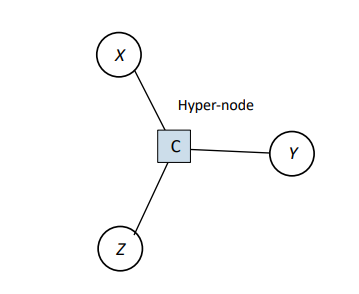
\includegraphics[scale=0.75]{5.png}
\end{center}
\subparagraph{Dual Graph transformation} Alternate way to convert a $n$-ary CSP to a binary one:
\begin{enumerate}
	\item Create a new graph in which there is one variable for each constraint in the original graph
	\item If two constraints share variables, they are connected by an arc corresponding to the constraint that the shared variables receive the same value
\end{enumerate}
Example: $Dom(x) = Dom(y) = Dom(z) = \{1,2,3\}$ with $C_1 = \{(x,y,z), x + y = z\} = \{(1,2,3), (2,1,3), (1,1,2)\}$ and $C_2 = \{(x,y), x < y\} = \{(1,2), (1,3), (2,3)\}$.
This will become $Dom(C_1) = \{(1,2,3), (2,1,3), (1,1,2)\}, Dom(C_2)=\{(1,2), (1,3), (2,3)\}$ and $R_{x,y} =$ constraint that $x$ and $y$ will receive the same values
\begin{center}
	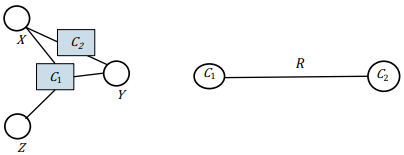
\includegraphics[scale=0.75]{6.png}
\end{center}
\paragraph{Related concepts} \begin{list}{}{}
	\item \textbf{Problem reduction techniques}: techniques for transforming CSP into an equivalent problem easier to solve or recognizable as insoluble
	\item \textbf{Enforcing local consistency}: the process of enforcing local consistency properties in a constraint graph causes inconsistent values to be eliminated. Different types of local consistency properties have been studied.
	\item \textbf{Constraint propagation/inference}: constraints are used to reduce the number of legal values for a variable, which in turn can reduce the legal value for another variable and so on\ldots
\end{list}
\subparagraph{Problem reduction} Reducing a problem means removing those constraints which appear in no solution tuples.\\
A CSP problem $P_1$ is reduced to $P_2$ when $P_1$ is equivalent to $P_2$, domains of variables in $P_2$ are subsets of those in $P_1$ and the constraints in $P_2$ are at least as restrictive as those in $P_1$.\\
These conditions guarantees that a solution in $P_2$ is also a solution in $P_1$.\\
\textbf{Problem reduction strategies} are of two types: removing redundant values from the domains of the variables or tightening the constraints so that fewer compound labels satisfy them (examples: if $x < y$ and $D_x = \{3,4,5\}, D_y = \{1, 2,4\}$ then those can be reduced to $D_x=\{3\}, D_y=\{4\}$.\\
Constraints are sets, this means removing redundant compound labels from the set. If the domain of any variable or any constraint is reduced to an empty set, then the problem is \textbf{unsolvable}.\\
Problem reduction is also called consistency checking or maintenance, since it relies on establishing local consistency properties.\\\\
\textbf{Local consistency properties}: node consistency, arc consistency, path consistency, k-consistency, forward checking.\\
All these operations do not change the set of solutions, do not necessarily solve a problem but, used with search, will make the search more efficient by pruning the search tree.
\begin{list}{}{} 
	\item \textbf{Node/Domain consistency}: a node is consistent if all the values in its domain satisfy unary constraints on the associated variable. A constraint network is node-consistent if all the nodes are consistent.\\
	Given a unary constraint on $x_i$, $C_i = \langle(x_i), R_i\rangle$ then node consistency $D_i \subseteq R_i$ and can be enforced by reducing the domains of the variables $D_i \leftarrow D_i \cap R_i$ (this is the NC-1 algorithm, $O(d\cdot n)$)
	\item \textbf{Arc consistency}: a variable is arc-consistent if every value in its domain satisfies the binary constraints of this variable with other variable. $x_i$ is arc-consistent with respect to $x_j$ if for every value in its domain $D_i$ there is some value in the domain $D_j$ that satisfies the binary constraint on the arc $(x_i, x_j)$\\
	Example, $X = \{x, y\}$, $D_x = D_y = \{0,1,2,3,4,5,6,7,8,9\}$ and constraint $\langle(x,y), x=y^2\rangle$. Considering arc $x \rightarrow y$, it can be made consistent by reducing $D_x$ to $\{0,1,4,9\}$. Considering $y \rightarrow x$, can be made consistent by reducing $D_y$ to $\{0,1,2,3\}$, making the entire edge consistent.
\end{list}
\paragraph{Arc Consistency Algorithm (AC-3)} It maintains a queue of arcs to consider, initially all the arcs in CSP. An edge produces two arcs. AC-3 pops off an arc $(x_i, x_j)$ from the queue and makes $x_i$ arc-consistent with respect to $x_j$: \begin{list}{}{}
	\item If this step leaves $D_i$ unchanged, the algorithm just moves on to the next arc
	\item If $D_i$ is made smaller, then we need to add to the queue all arcs $(x_k, x_j)$ where $x_k$ is a neighbor of $x_i \neq x_j$
	\item If $D_i$ becomes empty, then we conclude that the CSP has no solution
\end{list}
When there are no more arcs to consider, we have finished: we are left with a CSP equivalent to the original but smaller.\\
With a CSP of $n$ variables, each with domain size at most $d$ and $c$ binary constraints (arcs):
\begin{list}{}{}
	\item Checking consistency of an arc can be done in $O(d^2)$ time
	\item Each arc $(x_i, x_j)$ can be inserted in the queue only $d$ times (because $x_i$ has at most $d$ values to delete)
	\item We have $c$ arcs to consider, so complexity is $O(c\cdot d^3)$, polynomial time
\end{list}
The AC-4 algorithm is an improved version of AC-3, based on the notion of support that doesn't need to consider all the incoming arcs. More information is kept, but complexity is $O(c\cdot d^2)$.
\subparagraph{Example} $A, B, C \in \{1,2,3,4\}, A < B, A > C$\\
\begin{center}
\begin{tabular}{c c c}
	Queue & Arc & Arc domain\\
	\hline
	$\{(A,B), (B, A), (A, C), (C, A)\}$ & & \\
	$\{(B, A), (A, C), (C, A)\}$ & $(A,B)$ & $A \in \{1,2,3,\not 4\}$ \\
	$\{(A,C), (C, A)\}$ & $(B, A)$ & $B \in \{\not 1, 2, 3, 4\}$\\
	$\{(C, A)\}$ & $(A, C)$ & $A \in \{\not 1, 2, 3\}$\\
	$\{(B,A), (C, A)\}$ & & \\
	$\{(C, A)\}$ & $(B, A)$ & $B \in \{\not 2, 3, 4\}$\\
	$\{\}$ & $(C, A)$ & $C \in \{1, 2, \not 3,\not 4\}$\\
\end{tabular}
\end{center}
At the end $A\in\{2,3\}, B\in\{3,4\}, C\in\{1,2\}$
\paragraph{Directional Arc Consistency} DAC is defined with reference to a total ordering of the variables. A CSP is DAC under an ordering of the variables if and only if for every label $\langle x, a\rangle$ which satisfies the constraints on $x$ there exists a compatible label $\langle y,b\rangle$ for every label $y$ which is after $xc$ according to the ordering.\\
In the algorithm for establishing DAC (DAC-1) each arc is examined exactly once, by proceeding from last to the first in the ordiering, so the complexity is $O(c\cdot d^2)$. AC cannot always be achieved by running DAC-1 in both directions.
\paragraph{Generalized Arc Consistency} GAC, extension of AC-3 to handle $n$-ary constraints rather than just binary. A variable $x_i$ is GAC with respet to a $n$-ary constraint if for every value $v$ in the domain of $x_i$ there exists a tuple of values that is a member of the constraint and has its $x_i$ component equal to $v$.\\
For example, if $X, y, Z \in \{0,1,2,3\}$ and $X < Y < Z$, to make $C$ consistent we would have to eliminate $2, 3$ from the domain of $X$ because the constraint cannot be satisfied with $X=2$ or $X=3$.
\paragraph{Path Consistency} Arc consistency tightens down the domains using the arcs (binary constraints). Path consistency is a stronger notion: tightens the binary constraints by using implicit constraints that are inferred by looking at the triples of variables. A path of length 2 between variables $x_i, x_j$ is path-consistent with respect to a third intermediate variable $x_m$ if for every consistent assignment $\{x_i = a, x_j = b\}$ there is an assignment to $x_m$ that satisfies the constraints on $(x_i, x_m)$ and $(x_m, x_j)$. In relational algebra $R_{i,j}\subseteq\pi_{i,j}(R_{i,m}\bowtie D_m\bowtie R_{m,j})$\\
To achieve path consistency, $R_{i,j}\leftarrow R_{i,j}\cap\pi_{i,j}(R_{i,m}\bowtie D_m\bowtie R_{m,j})$ (algorithm name: PC-2). If all path of length 2 are made consistent, then all paths of any length are consistent.\\
Called path consistency because you can think of it as a path from $x_i$ to $x_j$ with $x_m$ in the middle.
\paragraph{Combining search and problem reduction} Problem reduction techniques are used in combination with search. The more effort one spends on problem reduction, the less effort one needs in searching.
\begin{center}
	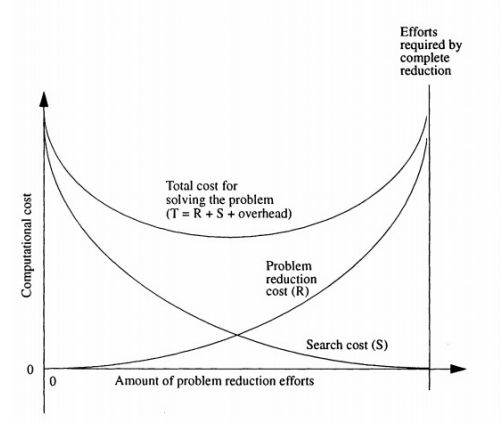
\includegraphics[scale=0.75]{7.png}
\end{center}
Most problems cannot be resolved by reduction alone, we must search for solutions and combine problem reduction with search. In this context we talk about \textbf{constraint propagation} or \textbf{inference}. A classical incremental formulation of CSP as a search problem is:
\begin{list}{}{}
	\item States are partial assignments
	\item Initial state: empty assignment
	\item Goal state: complete assignment that satisfy all constraints
	\item Actions: assign to a specific unassigned variable $x_i$ a value $\in D_i$
\end{list}
Branching factor: $d$, with $d$ maximum cardinality of the domains. Number of leaves: $d^n$, with $n$ number of variables. $n$ finite $\Rightarrow$ space graph finite.
\paragraph{CSP as search: simplifications} We can exploit \textbf{commutativity}. A problem is commutative if the order of application of any given set of action has no effect on the outcome. In this case, the order of the variable assignments does not change the result.\\
We can consider a single variable for assignment at each step, so the branching factor is $d$ and the number of leaves id $d^n$. We can also exploit depth limited search: \textbf{backtracking search} with depth limit $n$.\\
Search strategies:
\begin{list}{}{}
	\item \textbf{Generate and Test}: generate a full solution and test it, not the best
	\item \textbf{Anticipated Control}: after each assignment we check the constraint, if some is violated we backtrack to previous choices (undoing the assignment)
\end{list}
\paragraph{Backtracking search algorithm}  %TODO code
\paragraph{Heuristics and search strategies}
\begin{list}{}{}
	\item \texttt{SELECT-UNASSIGNED-VARIABLE}: which variable should be assigned next?
	\item \texttt{ORDER-DOMAIN-VALUES}: in which order should the values be tried?
	\item \texttt{INFERENCE}: what inference should be performed at each step?\\
	Techniques for \textbf{constraint propagation} (local consistency enforcement) can be used
	\item \texttt{BACKTRACKING}: where to back up to? When the search ends up in an assignment that violates a constraint, can the search avoid repeating this failure? Forms of \textbf{intelligent backtracking}
\end{list}
\subparagraph{Choosing the next variable}\begin{list}{}{}
	\item \textbf{MRV} (minimnum remaining values): variable with fewest "legal" remaining values
	\item \textbf{Degree heuristic}: variable involved in the largest number of constraints
\end{list}
\subparagraph{Choosing value} \begin{list}{}{}
	\item \textbf{Least constaint variable}: prefer the variable rules out the fewest choices
\end{list}
Note that in choosing the variable, a fail-first strategy helps in reducing the amount of search by pruning large parts of the tree earlier. In the choice of value, a fail-last approach works best in CSP where the goal is to find \textit{any} solution. This is not effective if we are looking for all solutions or no solution exists.
\subparagraph{Interleaving search and inference} One of the simplest form of inference propagation is \textbf{forward checking}: efficient constraint propagation, weaker than other forms. Whenever $X$ is assigned, FC process establishes arc consistency of $X$ for the arcs connecting neighbor nodes. For each unassigned $Y$ connected to $X$, delete from $Y$'s domain any value inconsistent with the value assigned to $X$.
\subparagraph{Constraint learning} When the search is at a contradiction, we know that some subset of the conflict set is responsible. Constraint learning is the idea of finding a minimum set of variables from the conflict set that causes the problem: the no-good set. We record the no-good set either by adding a new constraint to CSP or by keeping a separate cache of no-goods. This way we do not repeat the no-good state.

\paragraph{Local search} Requires a complete state formulation, keep in memory only current state to improve it iteratively and does not guarantee to find a solution even if it exists (\textbf{not complete}).\\
Used when space too large for systematic search and we need to be very efficient. Also when we need to provide a solution but it's not important to produce solution path. Also when we know in advance that a solution exists.
\subparagraph{Local search methods for CSP} Complete state formulation: we start with a complete random assignment, and we try to fix it until all the constraints are satisfied.\\
Local methods are very efficient for large scale problems where the solutions are densely distributed in the space. A basic algorithm is:
\begin{verbatim}
function Local_search(V, Dom, C) returns a complete & consistent assignment
Inputs: V: a set of variables
Dom: a function such that Dom(x) is the domain of variable x
C: set of constraints to be satisfied
Local: A (complete assignement) an array of values indexed by variables in V

repeat until termination
for each variable x in V do # random initialization or random restart
A[x] := a random value in Dom(x)
while not stop_walk( ) & A is not a satisfying assignment do # local search
Select a variable y and a value w in Dom(y), w != A[y] # a successors
A[y] := w # change a variable
if A is a satisfying assignment then return A # solution found
\end{verbatim}
this can be specialized, two extreme versions are: \textbf{random sampling} (no walking done to improve solution, so \texttt{stop\_walk} always \texttt{true}, just generating random assignments and testing them) or \textbf{random walk} (no restarting is done, so \texttt{stop\_walk} always \texttt{false})
\subparagraph{Heuristic Local Search} Inject heuristics in the selection of the variable and the value by the means of an evaluation function (in CSP, $f$ = \# violated constraints or conflicts, perhaps with weights).\\
\textbf{Iterative best improvement}: choose the successor that most improves the current state according to an evaluation function $f$. Moves to best successor even if worse than current state, may be stuck in loops, not complete.
\subparagraph{Stochastic Local Search} Adds randomness, escapes local minima:\begin{list}{}{}
	\item \textbf{Random restart} is a global random move: the search starts from a completely different part of the search state
	\item \textbf{Random walk} is a local random move: random steps are taken interleaved with the optimizing steps
\end{list}
There are possible variants \begin{list}{}{}
	\item Most improving step: selects a variable-value pair that makes the best improvement. Needs to evaluate all of them, needing strategies for efficient computation
	\item Two stage choice: select the variable that participates in most conflicts, then the value that minimizes conflicts (or a random value)
	\item Any conflict: choose a conflicting variable at random, select the value that minimizes conflicts (or a random value)
\end{list}
\paragraph{CSP: Min-Conflict Heuristic} All the local search techniques are candidate for CSP, some have proved especially effective. Min-conflict heuristics is widely used and also quite simple:
\begin{list}{}{}
	\item select a variable at random among the conflicting variables
	\item select the value that results in the \textbf{minimum number of conflicts} with other variables
\end{list}
%TODO algorithm
\subparagraph{Improvements} Usually many plateaus, possible improvements:
\begin{list}{}{}
	\item \textbf{Tabu Search}: local search has no memory, the idea is keeping a small list of the last $t$ steps and forbidding the algorithm to change the value of a variable whose value was changed recently. This is meant to prevent cycling among assignments, and $t$ is called \textbf{tenure}
	\item \textbf{Constraint Weighting}: concentrates the search on important constraints. We assign a numeric weight to each constraint, initially 1. The weight is incremented each time the constraint is violated: goal is choose the variable and value which minimizes the weights of the violated constraints.
\end{list}
\subparagraph{Alternatives}\begin{list}{}{}
	\item \textbf{Simulated Annealing}: allows downhill moves at the beginning of the algorithm and slowly \textit{freezes} this possibility
	\item \textbf{Population based methods}
	\begin{list}{}{}
		\item \textbf{Local Beam Search}: proceed with the $k$ best successors according to the evaluation function
		\item \textbf{Stochastic Local Beam Search}: selects $k$ of the individuals at random with a probability that depends on the evaluation function
		\item \textbf{Genetic Algorithms}\ldots
	\end{list}
\end{list}
\subparagraph{Online search} Another advantage of local search methods is that they can be used in an online setting when the problem changes dynamically.
\subparagraph{Evaluating randomized algorithms} Randomized algorithms are difficult to evaluate since they output a different result and a different execution time each time they run. We take the runtime distribution, which shows the number of runs in which the algorithm solved the problem within a given number of steps.\\
A randomized algorithm can be run multiple times with random restart, increasing the probability of success. An algorithm that succeeds with probability $p$ run $n$ times will found a solution with probability $1 - (1-p)^n$ with $(1-p)^n$ the probability of failing $n$ times.
\paragraph{Independent sub-problems} When problems have a specific structure, which is reflected in properties of the constraint graph, there are strategies for improving the process of finding a solution. A first obvious case is that of independent subproblems, for examples in the map coloring problem, a country which is not connected to another country (in the image, $T$) can be colored \textit{independently} from the others, and any solution for that country combined with any solution for the other countries yields a solution for the whole map.
\begin{center}
	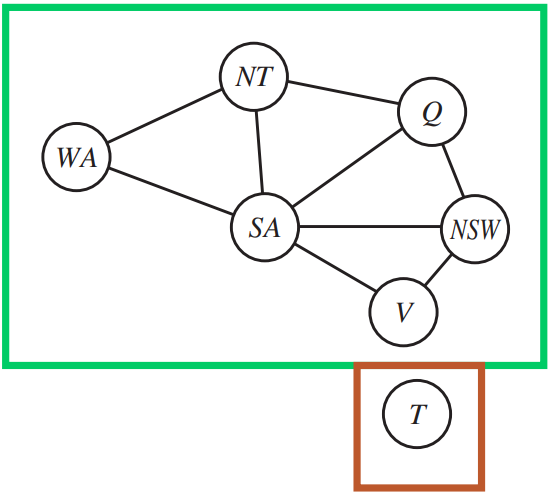
\includegraphics[scale=0.75]{8.png}
\end{center}
Formally, each \textbf{connected component} of the constraint graph corresponds to a subproblem $CSP_i$. If an assignment $S_i$ is a solution of $CSP_i$ then $\bigcup_i S_i$ is a solution of $\bigcup_i CSP_i$.
\subparagraph{Complexity} The saving in computational time is dramatic. With $n$ variables and $c$ variables for subproblems, we have $\frac{n}{c}$ independent subproblems. Given $d$ size of the domain, solving one subproblem costs $O(d^c)$ and solving all of them costs $O(d^c\frac{n}{c})$, \textbf{linear} in the number of variables $n$ rather than $O(d^n)$ exponential!\\
Dividing a boolean CSP with 80 variables into 4 subproblems reduces the worst case solution time from the lifetime of the Universe down to less than a second.
\paragraph{The structure of problems: trees}
\begin{center}
	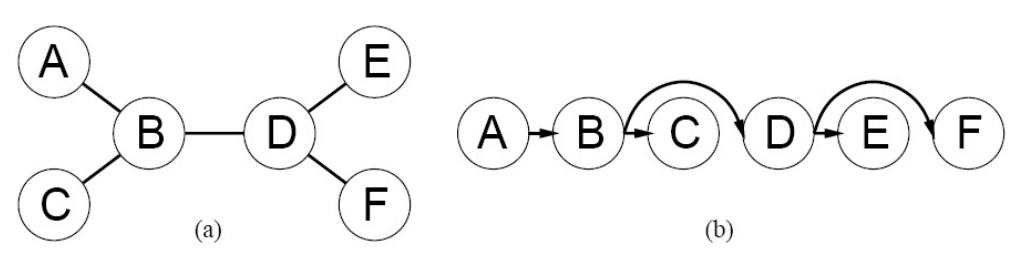
\includegraphics[scale=0.5]{9.png}
\end{center}
In a tree-structured graph, two node are connected by only one path: we can choose any variable as root of the tree. Chosen a variable as root, for example $A$, the tree induces a topological sort on the variables: children of a node are listed after their parent.
\subparagraph{Directional Arc Consistency} A CSP constraint graph is defined to be directionally arc-consistent under an ordering of variables $X_1,\ldots,X_n \Leftrightarrow$ every $X_i$ is arc-consistent with each $X_j$ for $j>i$.\\
We can make a tree-like graph directionally arc-consisten in one pass over the $n$ variables: each step must compare up to $d$ possible domain values for two variables (so $d^2$) for a total time of $O(nd^2)$
\subparagraph{Tree-CSP solver}\begin{enumerate}
	\item Proceeding from $X_n$ to $X_2$, make the arcs $X_i\rightarrow X_j$ DAC by reducing the domain of $X_i$ if necessary. This can be done in one pass
	\item Proceeding from $X_1$ to $X_n$, assign values to variables. There's \textbf{no need for backtracking} since each value for a father has at least one legal value for the child
\end{enumerate}
\paragraph{Reducing graphs to trees} For example, assigning a value to the node we want to remove and removing inconsistent values for other variables, then solve with tree-CSP solver.\\
In general not easy.
\subparagraph{Cutset conditioning} Domain splitting strategy, trying with different assignments: choose subset $S$ of CSP's variables such that the constraint graph becomes a tree: $S$ is called \textbf{cycle cutset}. For each consistent assignment to variables $\in S$: remove from the domains of remaining vars any inconsistent value, if the remaining CSP has a solution, return it together with the current assignment of $S$.\\
Time $O(d^c(n-c)d^2)$ where $c$ is size of the cycle cutset and $d$ size of the domain. We have to try each of the $d^c$ combinations of values for the variables $\in S$ and for each combination we must solve a tree problem of size $(n-c)$
\paragraph{Tree decomposition} The approach consists in a tree decomposition of the constraint graph into a set of connected sub-problems. Each of them is solved independently and the resulting solutions are combined cleverly.
\begin{center}
	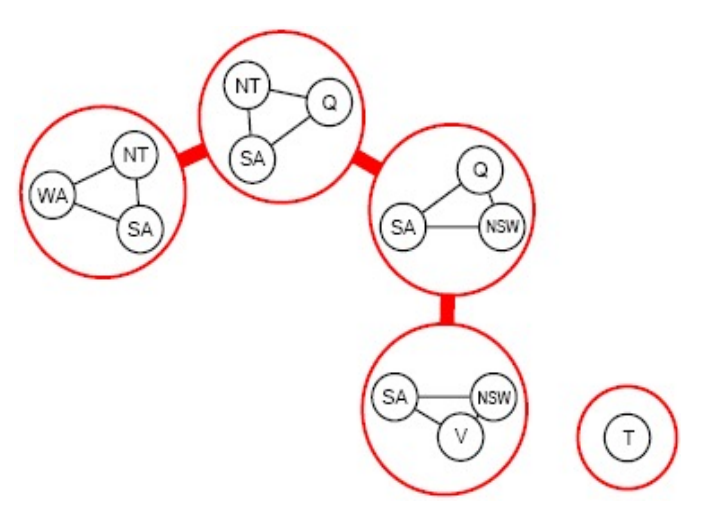
\includegraphics[scale=0.5]{10.png}
\end{center}
\begin{list}{}{}
	\item Every variable in the original problem must appear in at least one of the sub-problems
	\item If two variables are connected by a constraint, they must appear together int at least one of the subproblem, along with the constraint
	\item If a variable appears in two subproblems of the tree, it must appear in every subproblem along the path connecting those subproblems
\end{list}
1-2 ensure that all variables and constraints are represented. Condition 3 ensure that any given variable must have same value in every subproblem.
\subparagraph{Solving a decomposed problem} We solve each subproblem independently. If any problem has no solution then the original problem has no solution. For putting the solutions together, we solve a "meta-problem" as follows:
\begin{list}{}{}
	\item Each subproblem is a "mega-variable", whose domain is the set of all solutions for the subproblem.\\
	Es, Dom$(X_1) = \{($WA=r, SA=b, NT=g$),\ldots\}$
	\item The constraints ensure that the subproblem solutions assign the same values to the variables they share
\end{list}
The tree width of the decomposition is the size of the largest subproblem $-1$. Ideally we should find, among many possible ones, a tree decomposition with minimal tree width. NP-hard but heuristics exists.
\paragraph{Symmetry} Important factor for reducing the complexity of CSP problems. Value symmetry: the values does not really matter, for example different colors but there are 6 equivalent ways of satisfying the constraints. If $S$ is a solution to coloring $n$ var, then there are $n!$ solutions.\\
\textbf{Symmetry breaking constraints}: we impose an arbitrary ordering constraints that requires the values to be in alphabetical order. Breaking value symmetry has proved to be important and effective on many problems.
\subparagraph{Three approaches}
\begin{list}{}{}
	\item Reformulate the problem so that it has a reduced amount of symmetry, or none at all.
	\item Add symmetry breaking constraints before the search begins, making some symmetric solutions unacceptable while leaving at least one solution in each symmetric equivalence class
	\item Break symmetry dynamically during search
\end{list}
It's an active area of research.
\section{Knowledge Based Systems}
\subsection{Knowledge Representation and Reasoning}
Introducing an additional level of complexity in the representation of states. Knowledge based systems have rich representation languages and the ability to do inference (derive new knowledge). These languages rely on classical logic.\\
Other representation languages are proposed for inherent limitations in classical logic or for improving efficiency of inference.\\\\
\textbf{Knowledge Representation and Reasoning} (KR\&R) is the field of AI dedicated to representing information about the world in a form that a computer system can use to solve complex tasks. The class of systems that derive from this is called \textbf{knowledge based} (KB) systems/\textbf{agents}. A KB agent maintains a knowledgebase of facts expressed in a declarative language, and is able to perform automated reasoning to solve complex tasks.\\
The knowledgebase (KB) is the agent's representation of the world which is responsible for its intelligente behavior.\\\\
We will deal on how knowledge is represented and reasoned about, to derive new knowledge or decide actions. A separate important issue is how knowledge is acquired: hardcoded, obtained automatically\ldots and how it evolves maintaining its anchorage to the world.
\paragraph{Knowledge} What kind of knowledge? The emphasis is the relation between an agent and \textbf{facts that may be true or false in the world}. With $p$ proposition, something true or false: "John knows $p$", "John believes $p$", "John desires $p$", "John is confident that $p$"\ldots\\
Contrast with non-factual knowledge: knowing how ("John knows how to play the piano"), when, where ("John knows where the party is"), a person ("John knows Bill very well")\ldots\\
Represented knowledge is given a propositional account. Knowledge representation is about the use of formal symboli structures to represent a collection o propositions, believed by some agent. Not necessarily all of them.\\
\textbf{A representation is a surrogate}.
\begin{center}
	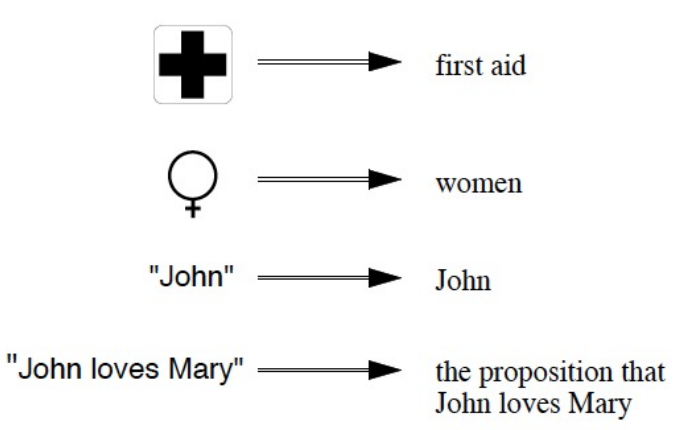
\includegraphics[scale=0.5]{11.png}
\end{center}
\paragraph{Reasoning} Is the formal manipulation of the symbols representing a collection of beliefs, to produce representations of new ones. Analogy with arithmetic. \textbf{Logical deduction} is a very well know example of reasoning.\\
Why reasoning? We would like the system to depend on what it believes and not what was explicitly stored. It's a question of economy of the representation.\\
Usually we need more than just DB-styled retrieval of facts in the KB. Explicit and implicit beliefs, logical entailment (KB $\vDash \alpha$).\\
Other forms of reasoning: \textbf{abductive reasoning} (given a causal relation $a\Rightarrow b$, from observing $b$ we can conjecture $a$: it's a way of providing an explanation) or \textbf{inductive reasoning} (from specific observation to a general rule)
\paragraph{The Knowledgebase Representation hypothesis} \textit{Any mechanically embodied intelligent process will be comprised of structural ingredients that
\begin{list}{}{}
	\item we, as external observers, naturally take to represent a propositional account of the knowledge that the overall process exhibits, and
	\item independent of such external semantic attribution play a formal but causal and essential role in engendering the behavior that manifests that knowledge
\end{list}}
Brian C. Smith, 1985\\\\
Putting it simply, we want AI systems that contain symbolic representations with two important properties:
\begin{list}{}{}
	\item We can understand those symbolic structures as propositions
	\item These symbolic structures determine the behavior of the system
\end{list}
Knowledge based systems have these properties.\\\\
Competing approaches: \textbf{procedural approach} (knowledge is embedded in programs) and \textbf{connectionist approach} (avoids symbolic representation and reasoning, instead models intelligent behavior by computing with networks of weighted links between artificial neurons)
\paragraph{Advantages of KB systems}
\begin{list}{}{}
	\item The try solving \textbf{open-ended tasks}, not per-compiled kind of behavior for specific tasks
	\item \textbf{Separation} of knowledge and "inference engine"
	\item \textbf{Extensibility}: we can extend the existing behavior by simply adding new proposition. \textbf{Knowledge is modular}, the reasoning mechanism does not change.
	\item \textbf{Understandability}: the system can be understood at knowledge level. Important for debugging, so we can debug faulty behavior by changing erroneous beliefs, and \textbf{accountability}, so that the system can explain and justify current behavior in terms of the knowledge used.
\end{list}
Representation and reasoning are intimately connected, in AI research. \textbf{The representation scheme must be expressive enough} to describe many aspects of complex worlds with symbolic structures. The reasoning mechanism needs to ensure that \textbf{reasoning can be performed efficiently enough}. There is a trade-off between these two concerns.\\
\textbf{Fundamental trade-off in knowledge representation and reasoning}: the more expressive the representation language is, the more complex is the reasoning. We want the best compromise.\\
The expressivity of representation language doesn't concern what \textit{can be said}, but what \textit{may be left unsaid}: it's related to the possibility of expressing uncertainty and incomplete information.\\
The complexity of inference regards the computational cost of deciding entailment (KB $\vDash \alpha$)
\subsubsection{Knowledge representation and classical logic}
Classical logic is propositional calculus (PROP) and first order predicate logic (FOL). We can understand KB systems at two different levels:
\begin{list}{}{}
	\item \textbf{Knowledge level}: representation language and its semantics, what can be expressed and what can be inferred
	\item \textbf{Symbol level}: computational aspects, efficiency of encoding, data structures and efficiency of reasoning procedure, including their complexity
\end{list}
%TODO PROP recap
\subsubsection{DPLL} Requires a formula in clausal form (conjunctive normal form, a conjunction of disjunctions of atomic formulas meaning "and outside or inside")\\
It enumerates, with a depth first strategy, all interpretations looking for a model (an interpretation that makes a set of formulas true), with three strategies:
\begin{list}{}{}
	\item Anticipated control: if one clause is false it backtracks, if one literal is true then the clause is satisfied
	\item Pure symbols heuristics: assign first pure symbols (symbols that appear everywhere with the same sign)
	\item Unit clauses heuristics: assign first unit clauses (only one literal)
\end{list}
%TODO FOL recap
\subsubsection{Unification algorithm} Computes the MGU by means of a rule-based equation-rewriting system. Initially the working memory (WM) contains the equality of the two expressions to be unified and the rules modify the equations in the WM. The algorithm terminates with a failure or when there are no applicable rules (success), so that the WM contains the MGU. The rules are:
\begin{list}{}{}
	\item $f(s_1,\ldots,s_n)=f(t_i,\ldots,t_n) \rightarrow s_1 = t_1, \ldots, s_n= t_n$
	\item $f(s_1,\ldots,s_n)=g(t_i,\ldots,t_m) \rightarrow$ fail when $f\neq g$ or $n\neq m$
	\item $x = x \rightarrow$ remove equation
	\item $t = x \rightarrow x = t$ (bring variable to the left)
	\item $x = t$, $x$ doesn't occur in $t \rightarrow$ apply $\{x/t\}$ to other equations
	\item $x = t$, $t$ is not $x$, $x$ occur in $t\rightarrow$ fail (\textbf{occur check})
\end{list}
Note: when comparing two different constants, we use the second rule as a special case where $n=m=0$ and we fail.
%KRR-2.pdf
\subsubsection{Knowledge Engineering \& Ontological Engineering} It's possible to discuss representation issues at two levels:
\begin{list}{}{}
	\item \textbf{Knowledge Engineering} is the activity to formalize a specific problem or task domain. It involves decisions about: what are the relevant facts and objects relations, which is the right level of abstraction and what are the queries to the KB (inferences)
	\item \textbf{Ontological Engineering} seeks to build general-purpose ontologies which can be reused in any special-purpose domain (with additional domain-specific axioms).
\end{list}
Sometimes it's useful to reduce $n$-ary predicates to 1-place predicates and 1-place functions: this involves creating new individuals and new functions for properties/roles and it's typical of description logics/frame languages.\\
For example Purchase(john, sears, bike, \$200), we can introduce individuals for purchase objects and functions for roles (\textbf{reification}): Purchase(p23)$\wedge$agent(p23)=john$\wedge$object(p23)=bike$\wedge$source(p23)=sears$\wedge$amount(p23)=\$200\ldots\\
This allows Purchase to be described at different levels of detail.
\paragraph{Representing common sense} The use of KR languages and logic in AI is representing common sense knowledge about the world, rather than mathematics or properties of programs. Common sense knowledge is difficult since it comes in different varieties. It requires formalisms able to represent actions, events, time, physical objects, beliefs\ldots categories that occur in many different domains. We will explore FOL as a tool to formalize different kinds of knowledge.
\begin{center}
	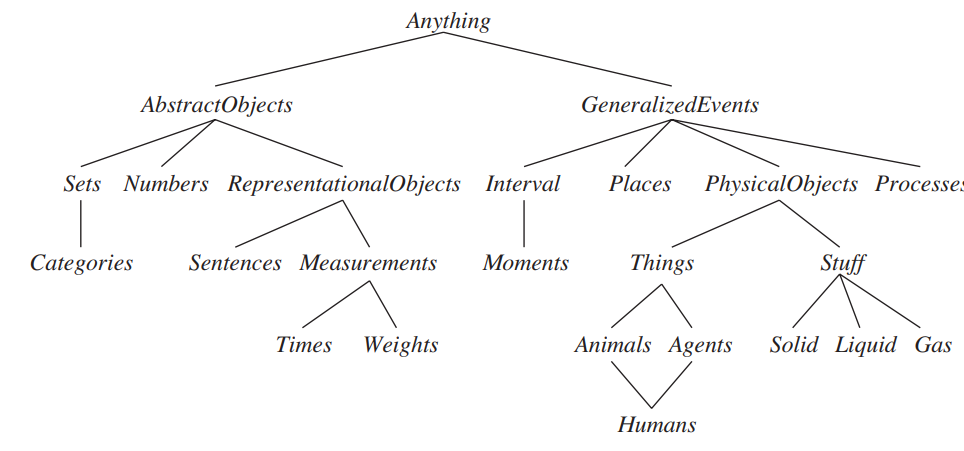
\includegraphics[scale=0.5]{12.png}
\end{center}
A general ontology organizes everything in the world into a hierarchy of categories.
\paragraph{Properties} A general-purpose ontology should be applicable in any special-purpose domain, with the addition of domain-specific axioms. In any non-trivial domain, different areas of knowledge must be combined because reasoning and problem solving could involve several areas simultaneously.\\
It's difficult to construct one single best ontology: every ontology is a treaty, a social agreement, among people with some common interest in sharing. An upper ontology is like an object oriented programming framework (reuse).
\paragraph{Categories and objects} Much reasoning takes place at the level of categories: we can infer category membership from the perceived properties of an object, and the use category information to derive specific properties of the object.\\
There are two choices for representing categories in first-order logic:
\begin{list}{}{}
	\item Predicates: categories are unary predicates that we assert of individuals\\
	Example: WinterSport(Ski), $\forall\:x$ WintersSport($x$) $\Rightarrow$ Sport($x$)
	\item Objects: categories are objects that we talk about (\textbf{reification})\\
	Examples: Ski $\in$ WinterSports, WinterSports $\subseteq$ Sports
\end{list}
This way we can organize categories into taxonomies, define disjoint categories, partitions\ldots and use specialized inference mechanisms, such as \textbf{inheritance}. Description logic takes this approach.
\subparagraph{PartOf} PartOf to say that one thing is part of another. Composite objects can be seen as part-of hierarchies, similar to the Subset hierarchy.\\
PartOf is trainsitive, PartOf($x,y)\wedge$ PartOf$(y,z)\Rightarrow$ PartOf$(x,z)$, and reflexive, PartOf$(x,x)$
\subparagraph{BunchOf} BunchOf is a composite object with definite parts but no particular structure. BunchOf(\{Apple1, Apple2, Apple3\}) not to be confused with the set of the 3 apples.\\
BunchOf(\{$x$\}) = $x$ and each element of category $S$ is part of BunchOf($S$). Also BunchOf($S$) is part of any object that has all the elements of $S$ as parts ($\forall\:y[\forall\:x\:\:x\in S\Rightarrow$ PartOf$(x,y)]\Rightarrow$ PartOf(BunchOf$(S),y)$)
\subparagraph{Qualitative Measures} Measures (weight, mass, cost\ldots) are represented as unit functions that take the number as argument (for example: Centimeters(2.54))\\
The measures can be ordered, which enables us to do qualitative inference and is typical of the field of qualitative physics.
\subparagraph{Objects vs Stuff} Objects are countable, while stuff are mass objects: water, energy, butter\ldots\\
Any part of a stuff is still stuff, example with Butter: $b\in$ Butter $\wedge$ PartOf$(p,b)\Rightarrow p\in$ Butter\\
Also stuff has a number of intrinsic properties (color, density, high-fat content\ldots) shared by all its subparts, but no extrinsic properties (weight, length, shape\ldots). It is a substance.
\subsubsection{Situation Calculus} Representation and reasoning about states and actions. The situation calculus is a specific ontology in FOL dealing with actions and change:
\begin{list}{}{}
	\item \textbf{Situations}: snapshots of the world at a given instant in time, the result of an action
	\item \textbf{Fluents}: time dependent properties and relations
	\item \textbf{Actions}: performed by an agent, but also events
	\item \textbf{Change}: how the worlds changes as a result of an action
\end{list}
The situation calculus is the formalization in FOL of this ontology. An example: the blocks world, there are blocks on a table and the goal is to reach a given arrangement of the blocks by stacking them on top of each other.
\begin{center}
	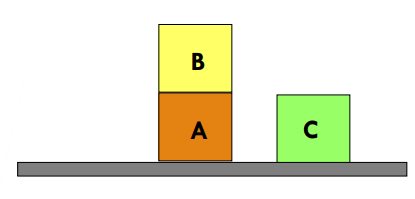
\includegraphics[scale=0.75]{13.png}
\end{center}
\begin{list}{}{}
	\item \textbf{States}: arrangements of blocks on a table
	\item \textbf{Initial State} and \textbf{Goal State}: a specific arrangement of blocks
	\item \textbf{Actions}:
	\begin{list}{}{}
		\item \textbf{Move}: move block $x$ from block $y$ to block $z$, provided $x$ and $z$ are free
		\item \textbf{Unstack}: move block $x$ from $y$ to the table, $x$ must be free
		\item \textbf{Stack}: move block $x$ from the table to $y$, $y$ must be free
	\end{list}
\end{list}
Can be formalized as:
\begin{list}{}{}
	\item \textbf{Situations}: constants $s,s_0,s_1,\ldots$ and functions denoting situations
	\item \textbf{Fluents}: predicates or functions that vary from a situation to another.\\
	On, Table, Clear\ldots are Fluents, so for example On($a,b$) becomes On($a,b,s$)
	\item \textbf{Actions}: modeled as functions\\
	Move($a,b,c$) is a function representing the action of moving block $A$ from $B$ to $C$. It's an instance of the generic operator/function Move. Same thing for Unstack($a,b$) and Stack($a,b$)
\end{list}
Situations as results of actions: function Result : $A\times S\rightarrow S$, so $s_1 =$ Result(Move($b,a,c),s_0$) denotes the situation resulting from the action Move($b,a,c$) executed in $s_0$. Then we can assert, for example, On($b,c,$Result(Move($b,a,c),s_0))$
\begin{center}
	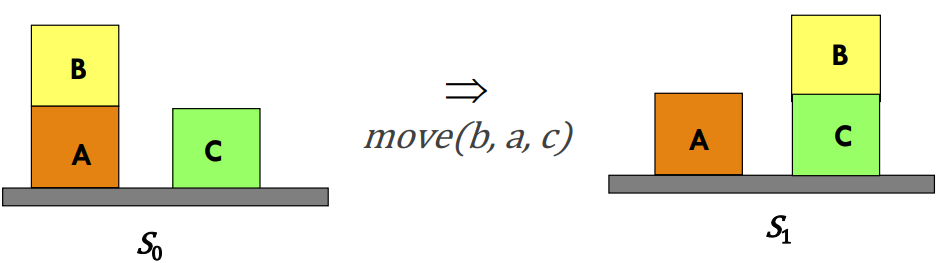
\includegraphics[scale=0.5]{14.png}
\end{center}
This can be applied to sequences of actions, too. Result : $[A^*]\times S \rightarrow S$
\begin{list}{}{}
	\item Result($[],s)=s$
	\item Result($[a\:|\:$seq$],s) =$ Result(seq, Result$(a,s))$
\end{list}
In general Result($[a_1,a_2,\ldots,a_n],s_0) =$ Result$(a_n$, Result($a_{n-1}$, \ldots Result($a_2$, Result($a_1, s_0$))\ldots))
\paragraph{Formalizing actions} We need \textbf{possibility axioms}, with the structure preconditions $\Rightarrow$ possibility, for example
\begin{list}{}{}
	\item On$(x,y,s)\wedge$ Clear$(x,s)\wedge$ Clear$(z,s)\wedge x\neq z \Rightarrow$ Poss(Move$(x,y,z),s)$
\end{list}
We also need \textbf{effect axioms} such as
\begin{list}{}{}
	\item Poss(Move$(x,y,z),s)\Rightarrow$ On($x,z,$ Result(Move$(x,y,z),s))\wedge$ Clear($y,$ Result(Move$(x,y,z),s))$
\end{list}
This is a specification of the direct effects of the action, what changes. But it's not enough: is $y$ on the table in the new situation? Is $x$ free?\\
We have a big problem: in the new situation we don't know anything about properties that were not influenced at all by the action, and these properties are the majority. This is the \textbf{frame problem}.
\paragraph{Frame problem and frame axioms} The frame problem is one of the most classical AI problems. The name comes from an analogy with the animation world, where the problem is to distinguish the background (the fixed part) from the foreground (the things that change) from one frame to the other.\\
Let's fix the problem with frame axioms: Frame axioms for Clear with respect to Move
\begin{list}{}{}
	\item A block stays free unless the Move action is putting something on it\\
	Clear$(x,s)\wedge x\neq w\Rightarrow$ Clear($x,$ Result(Move$(y,z,w),s))$
	\item A block remains not free unless it is not freed by a Move action\\
	$\neg$Clear$(x,s)\wedge x\neq z\Rightarrow$ $\neg$Clear$(x,$ Result(Move$(y,z,w),s))$
\end{list}
And similarly for each pair Fluent-Action: too many axioms, \textbf{representational frame problem}.
\paragraph{Successor-State axioms} We can combine preconditions, effects and frame axioms to obtain more compact representation for each fluent $f$. The schema is this:\begin{center}
\begin{tabular}{r l l}
$f$ true after $\Leftrightarrow$ & [\textit{preconditions before} and & \textit{preconditions}\\
& \textit{an action made $f$ true}] or & \textit{effect}\\
& [$f$ \textit{was true before and no action made it false}] & \textit{frame axioms}
\end{tabular}
\end{center}
An example with Clear:\begin{center}
\begin{tabular}{r l l}
Clear$(y$, Result$(a,s))$ $\Leftrightarrow$ & [On$(x,y,s)\wedge$ Clear$(x,s)\wedge$ Clear$(z,s)\wedge x\neq z \wedge a =$ Move$(x,y,z)$] $\vee$ & \textit{effect}\\
& [On($x,y,s)\wedge$ Clear$(x,s)\wedge(a =$ Unstack$(x,y,))$] $\vee$ & \textit{effect}\\
& [Clear$(y,s)\wedge(a\neq$ Move$(z,w,y))\wedge(a\neq$ Stack$(z,y))$] & \textit{frame}
\end{tabular}
\end{center}
\paragraph{Related problems} The \textbf{representational frame problem} is considered more or less solved.
\subparagraph{Qualification problem} In real situations it is almost impossible to list all the necessary and relevant preconditions.
\subparagraph{Ramification problem} Among derived properties, which ones persist and which ones change?\\
Objects on a table are in the room where the table is. If we move the table from one room to another, object on the table must also change their location. Frame axioms could make the old location persist for objects.
\paragraph{Uses of situations calculus} \begin{list}{}{}
	\item \textbf{Planning}: finding a sequence of actions to reach a certain goal condition $G$\\
	KB$\vDash\:\exists\:a\:\:G$(Result$(a,s_0))$ where $a = [a_1,\ldots,a_n]$
	\item \textbf{Projection}: given a sequence of actions and some initial situation, determine what it would be true in the resulting situation.\\
	Given $\phi(s)$ determine whether KB$\vDash\:\phi($Result$(a,s_0))$ where $a = [a_1,\ldots,a_n]$
	\item \textbf{Legality test}: checking whether a given sequence of actions $[a_1,\ldots,a_n]$ can be performed starting from an initial situation.\\
	KB$\vDash\:$Poss$(a_i,$ Result$([a_1,\ldots,a_{i-1}],s_0))$ for each $i\:|\:1\leq i\leq n$\\
	For example Result(Pickup($b_2$), Result(Pickup$(b_1),s_0))$ is not a legal situation because the robot can hold only one object.
\end{list}
\paragraph{Non-Monotonic approach} What we would need is the ability to formalize a notion of \textbf{persistence}: \textit{in the absence of information to the contrary, things remain as they were}".\\
This leads out of classical logic, because it violates the \textbf{monotonicity property} of classical logic. The \textbf{closure assumption} we used is already an ad hoc form of completion and we will see more of this strategy in non-monotonic reasoning.\\
In planning, specialized languages that makes more assumptions and are more limited in their expressivity.
\paragraph{Limits of situation calculus} Single agent, actions are discrete and instantaneous (no duration in time), they happen one at a time (no concurrency, no simultaneous actions) and only primitive actions (no way to combine, conditionals, iterations,\ldots)\\
The \textbf{event calculus} is introduced to handle such cases: it's based on events, points in time, intervals rather than situations.
\subsubsection{Event Calculus}
\begin{list}{}{}
	\item A Fluent is an object (represented by a function)\\
	To assert that a Fluent is true at some point in time $t$, we use the predicate $T($true$)$
	\begin{list}{}{}
		\item $T$(At(Shankar, Berkley)$, t)$
		Where  At(Shankar, Berkley) is a term, $t$ a time
		\item $T$(At(Shankar, Berkley)$, i)$
		With $i = (t_1, t_2)$ being a time interval
	\end{list}
	\item Events are described as instances of event categories. The event $E_1$ of Shankar flying from San Francisco to Washington is described as $E_1\in$ Flyings $\wedge$ Flyer$(E_1,$ Shankar$)\wedge$ Origin$(E_1,$ SF$)\wedge$ Destination$(E_1,$ W)
	\item To assert that an event happens during an extended period of time, we say Happens($e,i$)
\end{list}
\subsection{Nonmonotonic reasoning}
Classical entailment is monotonic: if KB$\vDash a$ then KB $\cup \{b\}\vDash a$ (KB$\wedge b\vDash a$)\\
Failures of monotonicity are widespread in commonsense reasoning. It seems that humans often "jump to conclusions" when they think it's safe to do so (when they lack information to the contrary). These conclusions are only "reasonable" given what you know, rather than classically entailed.\\
Most of the inference we do is defeasible: additional information may lead to retract those tentative conclusions. Anytime the set of beliefs does not grow monotonically when new evidence arrives, the monotonicity property is violated. Including defeasible reasoning leads us to consider \textbf{nonsound inferences}.
\paragraph{Common instances of nonmonotonic reasoning} \begin{list}{}{}
	\item \textbf{Default reasoning}: reasonable assumptions unless evidence of the contrary\\
	Car parked on the street: you assume it has for wheels even if you can only see two\\
	Also, prototypes: birds fly, tomatoes are red\ldots
	\item \textbf{Persistence}: things stay the same, according to the principle of inertia, unless we know they change
	\item \textbf{Economy of representation}: only true facts are stored, false facts are only assumed
	\item \textbf{Reasoning about knowledge}: if you have $\neg$Know($p$) and you learn $p$\ldots
	\item \textbf{Abductive reasoning}: most likely explanations to known facts
\end{list}
\paragraph{Strictness of FOL universals} Universal rules (example: $\forall\:x\:\:(P(x)\Rightarrow Q(x))$) express properties that apply to all instances: all or nothing. But most of what we learn about the worlds is in terms of generics rather than universals. Properties are not strict for all instances: genetic/manufacturing varieties, borderline cases (early ferry wheels vs modern ones, or violins vs toy violins\ldots), cases in exceptional circumstances\ldots\\
Listing all exceptions is not a viable solution: qualification problem in enumerating all exceptions, and similarly for general properties of individuals. The goal is to be able to say a $P$ is a $Q$ in general, normally, but not necessarily. It is reasonable to conclude $Q(a)$ given $P(a)$ unless there's a good reason not to.\\
This is what we call a default, and \textbf{default reasoning} the tentative conclusion. Three ways to approach the problem:
\begin{list}{}{}
	\item \textbf{Model Theoretic Formalizations} (CWA, Circumscription)\\
	Consist in a restriction to the possible interpretations, redefining the notion of entailment.
	\item \textbf{Proof Theoretic Formalizations} (Default logic, Autoepistemic logic)\\
	A proof system with non-monotonic inference rules. Autoepistemic logic (under the heading "logics for knowledge and beliefs")
	\item \textbf{Systems Supporting Belief Revision} (TMS, ATMS)
\end{list}
\paragraph{Closed Worlds Assumpion (CWA)} \textit{There are usually many more negative facts than positive facts}! Under CWA, only positive facts are stored, and any other basic fact is assumed false. It's used in deductive databases and in logic programming with negation as failure. Corresponds to a new version of entailment $\vDash_C$:
\begin{list}{}{}
	\item KB $\vDash_C a \Leftrightarrow$ CWA(KB) $\vDash a$\\
	Where CWA(KB) = KB $\cup\{\neg p\:|\:p$ ground atom and KB $\neq p\}$, the set of assumed beliefs\\
\end{list}
CWA(KB) is the completion under CWA of KB. CWA is a form of theory completion and is nonmonotonic.
\subparagraph{Consistent and complete knowledge} KB with consistent knowledge (satisfiable): $\not\exists\:a\:|$ KB$\vDash a\wedge$ KB$\vDash\neg a$, so there's no contradiction.\\
\textbf{Complete theory}: $\forall\:a$ KB$\vDash a\vee$ KB$\vDash\neg a$\\
Normally a KB has incomplete knowledge:
\begin{list}{}{}
	\item Let KB = $\{p\vee q\}$, then KB$\vDash (p\vee q)$ but KB$\not\vDash p$ and KB$\not\vDash \neg p$\\
	Also, for any ground atom not mentioned in KB, KB$\not\vDash r$ and KB $\not\vDash \neg r$
\end{list}
CWA can be seen as an \textbf{assumption about complete knowledge}, or a way to make a theory complete.\\
\textbf{Theorem}: $\forall\:a$ within the language, KB$\vDash_C a\vee$ KB$\vDash_C\neg a \Leftrightarrow$ CWA(KB)$\vDash a\vee$ CWA(KB)$\vDash\neg a$\\\\
CWA(KB) isn't always consistent when KB is consistent. Problems with disjunctions, for example: KB = $\{p\vee q\}$, CWA(KB) = KB$\cup\{\neg p, \neg q\}$ since KB $\not\vDash p$ and KB $\not\vDash q$, but KB$\cup\{\neg p, \neg q\}\vDash \neg(p\vee q)$ then CWA(KN) is inconsistent. The solution is to restrict CWA to atoms that are "uncontroversial": $p,q$ are controversial, $r$ isn't.\\
CWA limited in such a way is called Generalized CWA (GCWA), is a weaker form of completion than unrestricted CWA (the assumed beliefs are less)
\begin{list}{}{}
	\item GCWA: if KB $\vDash\{p\vee q_1,\ldots,\vee q_n\}$ and KB $\neg\vDash p$ then add $\neg p$, provided at least one ground atom $q_i$ is entailed by KB\\
	\textbf{Theorem} consistency of CWA: CWA(KB) is consistent $\Leftrightarrow$ whenever KB $\vDash(q_1\vee\ldots\vee q_n)$ then KB $\vDash q_i$ for some $i$.
\end{list}
Since it may be difficult to test the conditions of this theorem, the following \textbf{corollary} (which restricts the application of CWA) is also of practical importance: if the KB is made of Horn clauses and it's consistent, then CWA(KB) is consistent.\\
A clause is a disjuction of atomic formulas (positive and negative literals), and a Horn clause has \textit{at most} one positive literal.
\subparagraph{Vivid knowledgebase} A model is a vivid representation of the world. In a vivid KB we store a unique interpretation of the world (a consistent and complete set of positive literals) and answer questions retrieving from it. A vivid KB has the CWA built in.\\
If positive atoms are stored as a table, deciding if KB $\vDash_C a$ is like a DB retrieval. Instead of reasoning with sentences we reason about an analogical representation of the world, with these properties:
\begin{list}{}{}
	\item For each object of interest in the world, there is exactly one constant in KB that stands for that object.
	\item For each relationship of interest in the world, there is a corresponding predicate in the KB such that the relationship holds among certain objects in the world if and only if the predicate with the constants as arguments is an element of the KB.
\end{list}
\subparagraph{Extension to quantifiers} The application of the theorem of consistency depends on the terms that we allow as part of the language. The \textbf{Domain Closure Assumption} (DCA) may be used to restrict the constants to those explicitly mentioned in the KB. Under this restriction, quantifiers can be replaced by finite conjunctions and disjunctions.\\
The \textbf{Unique Names Assumption} (UNA) can be used to deal with terms equality.
\subparagraph{CWA in synthesis} CWA is the assumption that atomic formulas not entailed by the KB are assumed to be false. This is a normal assumption in databases. Formally, KB $\vDash_C a \Leftrightarrow$ KB $\cup\{\neg p\:|\:p$ ground atom and KB $\not\vDash p\}\vDash a$\\
The KN so augmented is \textbf{complete}: $\forall\:a$ KB $\vDash_C a$ or KB $\vDash_C \neg a$\\
\textbf{Consistency} requires a more restricted formulation of the assumed belief GCWA. If KB $\vDash \{p\vee q_1\ldots\vee q_n\}$ and KB $\not\vDash p$ then add $\neg p$ if at least one ground literal $q_i$ is entailed.\\
Query processing can be reduced as a combination of atomic queries.\\
Vivid knowledgebases store the plus part of a complete interpretation and make reasoning efficient (the augmentation reduces the possible models to one)
\paragraph{Circumscription} A more powerful and precise version of CWA, working also for FOL. The idea is to specify special \textbf{abnormality predicates} for dealing with exceptions.\\
For example, suppose we want to assert the default rule "birds fly":
\begin{list}{}{}
	\item All normal birds fly: $\forall\:x$ Bird$(x) \wedge\neg$Ab$_f(x)\Rightarrow$ Flies$(x)$
	\item We also have Bird(Tweety), Bird(Chilly), Chilly $\neq$ Tweety, $\neg$Flies(Chilly)\\
	We want to infer Flies(Tweety), but Tweetu could satisfy Ab$_f$ in some model
\end{list}
The idea is to \textbf{minimize abnormality}.\\
\textbf{Circumscription}: given the unary predicate Ab, consider only interpretation where I[Ab$_f$] is \textbf{as small as possible} relative to KB.
\subparagraph{Minimal Entailment} Let $P$ be a set of unary abnormality predicates. Let $I_1$ and $I_2$ two interpretations that agree on the values of constants and functions.\begin{list}{}{}
	\item \textbf{Ordering on interpretations}\\
	$I_1 < I_2 \Leftrightarrow$ same domain $\wedge\forall\:p\in P\:\:I_1[p]\subset I_2[p]$ holds
	\item \textbf{Minimal Entailment}\\
	KB $\vDash_\leq a \Leftrightarrow a$ is true in $I$ in every minimal model $I$\\
	Note: model ($I$[KB] = true) and minimal (there is no other interpretation $I' < I$ such that $I'$[KB] = true)\\
	$a$ doesn't need to be true in all interpretations satisfying KB but only in all those that minimize abnormalities.
\end{list}
\subparagraph{Issues} Although the default assumptions made by circumscription are usually weaker than those of the CWA, there are cases where they appear too strong.\\
A partial fix is to distinguish between $P$ (variable predicates) and $Q$ (fixed predicates), and ordering on interpretations differently for the two sets so that only predicates in $P$ are allowed to be minimized:
\begin{list}{}{}
	\item $\forall\:p\in P\:\:I_1[p] \subset I_2[p]$ holds
	\item $\forall\:q\in Q\:\:I_1[q] = I_2[q]$ holds
\end{list}
The problem is that we need to decide what to allow to vary.
\paragraph{Default Logic} We use rules to specify implicit beliefs. We distinguish explicit beliefs (axioms) from implicit beliefs (theorems).\\
Default logic KB uses two components: KB = (F, D)
\begin{list}{}{}
	\item F is a set of sentences (\textbf{facts})
	\item D is a set of \textbf{default rules} $\frac{\alpha : \beta}{\gamma}$\\
	Read it as: if you can infer $\alpha$ and it's consistent to assume $\beta$, then infer $\gamma$:
	\begin{list}{}{}
		\item $\alpha$ prerequisite
		\item $\beta$ justification
		\item $\gamma$ conclusion
	\end{list}
	Default rules where $\beta = \gamma$ are called normal defaults
\end{list}
\subparagraph{Extensions} How to characterize theorems/entailments? Cannot write a derivation, since don't know when to apply default rules, and no guarantee a unique set of theorems.\\
\textbf{Extensions}: set of sentences that are "reasonable" beliefs, given explicit facts and default rules. E is and extension of (F, D) $\Leftrightarrow$ for every sentence $\pi$, E satisfies the following:
$$\pi\in E\Leftrightarrow F\cup\Delta \vDash \pi\:\:\:\: \hbox{ where }\Delta=\left\{\gamma\:|\:\frac{\alpha : \beta}{\gamma}\in D, \alpha\in E, \neg\beta\not\in E\right\}$$
An extension E is the set of entailments of $F\cup\Delta$ where the $\Delta$ is the "suitable" set of assumptions given D.\\
Note that $\alpha$ has to be in E, not in F. This has the effect of allowing the prerequisite to be believed as the result of other default assumptions. Note also that this definition is not constructive.\\\\
\textbf{Theorem}: an extension of a default theory is inconsistent $\Leftrightarrow$ the original F is inconsistent.\\
In the following example the extension is unique, but in general a default theory can have multiple extensions.\\
Suppose KB is 
\begin{list}{}{}
	\item F = \{Bird(Chilly), Bird(Tweety), $\neg$Flies(Chilly)\}
	\item D = $\left\{\frac{\hbox{Bird}(x) : \hbox{Flies}(x)}{\hbox{Flies}(x)}\right\}$
\end{list}
then the unique possible extension is $\Delta = \{$Flies(Tweety)$\}$, since Bird(Tweety)$\in E$ and $\neg$Flies(Tweety)$\not\in E$.
\subparagraph{Properties} \begin{list}{}{}
	\item If a default theory has distinct extensions, they are \textbf{mutually inconsistent}.\\
	Example: F=\{A$\vee$B\}, D=$\left\{\frac{:\neg A}{\neg A}, \frac{:\neg B}{\neg B}\right\}$ then E$_1$=\{A$\vee$B, $\neg$A\}, E$_2$=\{A$\vee$B, $\neg$B\} are mutually inconsistent
	\item There are default theories with no extensions.\\
	Example: with D=$\left\{\frac{:\neg A}{\neg A}\right\}$, if F=\{\} then E=\{\}
	\item Every normal default theory has an extension
	\item Adding new normal default rules does not require the withdrawal of beliefs, even if adding new beliefs might. Normal default theories are semi-monotonic.
\end{list}
\subparagraph{Grounded Extensions} We have a problem that leads to a more complex definition of extension. Suppose F = \{\} and D=$\left\{\frac{:p}{\neg p}\right\}$. Then E = entailments of $\{p\}$ is an extension since $p\in E$ and $\neg p\not\in E$, but we have no good reason to believe $p$. The only support for $p$ is the default rule, which requires $p$ itself as a prerequisite. So the default should have no effect.\\
Desirable extension is only E = entailments of \{\}, that is to say all valid formulas. It's necessary a revision of the definition.\\
\textbf{Grounded extensions}: $\forall$ set $S$, let $\Gamma(S)$ be the least set containing $F$, closed under entailment and satisfying the default rules $$\frac{\alpha : \beta}{\gamma} \in D, \alpha\in \Gamma(S) \wedge \neg\beta\not\in S \Rightarrow \gamma\in \Gamma(S)$$
instead of $\neg\beta\not\in\Delta(S)$\\
A set $E$ is an extension of (F, D) $\Leftrightarrow E = \Gamma(E)$, i. e. E is a fixed point of the $\Gamma$ operator.
%KRR-4.pdf
\subsection{Knowledge and Beliefs}
Human intelligence is social: we need to negotiate and coordinate with others. In multi-agent scenarios we need methods for one agent to model \textbf{mental states} of other agents: high level representations of other agent's belief, intentions and goals may be relevant for acting.\\
By mental states we mean the relation of an agent to a proposition. \textbf{Propositional Attitudes} that an agent can have include Believes, Knows, Wants, Intends, Desires, Inform\ldots so called because the argument is a proposition. Propositional attitudes do not behave as regular predicates.
\paragraph{Referential Transparency} Suppose we try to assert "Lois knows that Superman can fly". Knows(Lois, CanFly(Superman))
\begin{list}{}{}
	\item What is "CanFly"? A predicate? A term?
	\item Since Superman = Clark, then we can reason as follows:\\
	(Superman = Clark) $\wedge$ Knows(Lois, CanFly(Superman)) $\vDash$ Knows(Lois, CanFly(Clark))
\end{list}
This property is called \textbf{referential transparency}: what matters is the object that the term names, not the form of the term. Important property for reasoning in classical logic.\\
Propositional attitudes like Believes and Knows require \textbf{referential opacity}: the terms used do matter, because an agent may not be aware of which terms are co-referential.
\subparagraph{Three approaches}
\begin{list}{}{}
	\item \textbf{Reification}: we remain within FOL, as we did for the situation calculus, using terms to represent propositions.\\
	Ex: Bel($a$, On($b,c$))
	\item \textbf{Meta-Lingustic representation}: we remain within FOL an represent proposition as strings.\\
	Ex: Bel($a$, "On($b,c$)")
	\item The problem in both of the previous approaches is connecting the reified version of the proposition (a function or a string) and the proposition itself
	\item \textbf{Modal Logics}: propositional attitudes are represented as \textbf{modal operators} in specialized modal logics, with alternative semantics. Modal operators are an extension of classical logical operators.\\
	Ex: B($a$, On($b,c$)) or B$_a$(On($b,c$)), K$_a$(On($b,c$)) to say that the agent $a$ believes/knows that block $b$ is on $c$.\\
	Classical logic has only one modality (modality of truth): $P$ is the same as saying "$P$ is true"
\end{list}
\paragraph{Modal Logics} Modal logic is about necessity and possibility.
\begin{list}{}{}
	\item $\square A$ it is necessary that $A$\ldots (with $\square$ being some sort of universal quantification over interpretations)
	\item $\lozenge A$ it is possible that $A$\ldots (with $\lozenge$ being some sort of existential quantification over interpretations)
\end{list}
The simplest logic is calle $K$, and results from adding the following to the principles of PROP:
\begin{list}{}{}
	\item \textbf{Necessitation Rule}: If $A$ is a theorem of $K$, then so is $\square A$
	\item \textbf{Distribution Axiom}: $\square (A\Rightarrow B) \Rightarrow (\square A \Rightarrow \square B)$
\end{list}
Logic $T$ adds axiom
\begin{list}{}{}
	\item[(M)] $\square A \Rightarrow A$
\end{list}
Can be relevant for some modal operators, but not for others. For example, Knows $A\Rightarrow A$ seems plausible, while Believes $A\Rightarrow A$ is not.\\
Logic $S4$ adds
\begin{list}{}{}
	\item $\square A \Rightarrow \square \square A$
\end{list}
Logic $S5$ adds
\begin{list}{}{}
	\item $\lozenge A \Rightarrow \square\lozenge A$
\end{list}
\subparagraph{World semantics} Semantics for modal logics is defined with reference to: a set $W$ of possible worlds and an \textbf{accessibility relation} $R$ between worlds.\\
A formula $A$ is now given an interpretation with reference to a possible world $w$: we write $I(A, w)$
\begin{list}{}{}
	\item[$\neg$] $I(\neg A, w)= T \Leftrightarrow I(A, w) = F$
	\item[$\Rightarrow$] $I(A\Rightarrow B, w)= T \Leftrightarrow I(A, w) = F\vee I(B, w) = T$
	\item[\vdots]
	\item[$\square$] $I(\square A, w)= T \Leftrightarrow\forall\:w'\in W\:|\: wRw'$ we have $I(A, w') = T$
	\item[$\lozenge$] $I(\lozenge A, w)= T \Leftrightarrow\exists\:w'\in W\:|\: wRw'$ we have $I(A, w') = T$
\end{list}
Different modal logics are defined according to the properties of the accessibility relation $R$ and corresponding axioms.
\subparagraph{Referential Transparency} Modal logics address this problem, since the truth of a complex formula does not depend on the truth of the components in the same world/interpretation. \textbf{Modal operator are not compositional}.\\
Modal logics for knowledge are easier than those of beliefs.
\subparagraph{Syntax for modal logic for knowledge} \begin{list}{}{}
	\item All the well formed formulas of ordinary FOL are also well formed formulas of the modal language
	\item If $\phi$ is a closed well formed formula of the modal language and $a$ is an agent, then Knows($a,\phi$) is a formula of the modal language
	\item If $\phi$ and $\psi$ are well formed formulas so are the formulas that can be costructed form thed with the usual logic connectives.
\end{list}
Some examples:
\begin{list}{}{}
	\item Knows(A$_1$, Knows(A$_2$, On(B, C))), A$_1$ knows that A$_2$ knows that B is on C
	\item Knows(A$_1$, On(B, C)) $\vee$ Knows(A$_1$, $\neg$On(B, C)), A$_1$ knows whether B is on C or not
	\item $\neg$Knows(A$_1$, On(B, C)), A$_1$ doesn't know that B is on C
\end{list}
\subparagraph{Properties of knowledge}\begin{list}{}{}
	\item One agent can hold false beliefs but \textbf{cannot hold false knowledge}.\\
	If an agent knows something then that must be true. \textbf{Knowledge is justified true belief}.
	\item An agent \textbf{doesn't know all the truths}: something may be true without the agent knowing it.
	\item If two formulas $\phi$ and $\psi$ are equivalent, not necessarily Knows(A, $\phi$) implies Knows(A, $\psi$)
\end{list}
The semantics of modal logic is given in terms of possible worlds, and specific accessibility relations among them, one for each agent.\\
An agent know a proposition just when that proposition is true in all the worlds accessible from the agent's worlds (those that the agent consider possible).\\
\textbf{Possible worlds} roughly correspond to contexts within interpretations. An accessibility relation is defined for agents and connects possible worlds: if Knows$(a, w_i, w_j)$ is satisfied, then world $w_j$ is accessible form world $w_i$ for agent $a$.\\
Possible world semantics:\begin{list}{}{}
	\item Regular well formed formulas (with no modal operators) are not simply true or false but they are true or false with reference to a possible world.\\
	$I(w_1, \phi)$ may be different from $I(w_2, \phi)$
	\item A modal formula Knows$(a, \phi)$ is true in $w \Leftrightarrow \phi$ is true in all the worlds accessible from $w$ for agent $a$.
	\item The semantics of complex formulas is determined by regular truth recursive rules.
\end{list}
Knows($a, \phi$) means that an agent $a$ knows the proposition denoted by $\phi$. "Not knowing $\phi$" in $w_0$, a specific world, is modeled by allowing some worlds, accessible by $w_0$, in which $\phi$ is true and some worlds in which $\phi$ is false.\\
For example, in this scenario Knows($a,P$) and Knows($a, \neg R$) in $w_0$ since $P$ and $\neg R$ are true in worlds $w_0,w_1,w_2,w_3$, but Knows($a, Q$) is false in $w_0$.
\begin{center}
	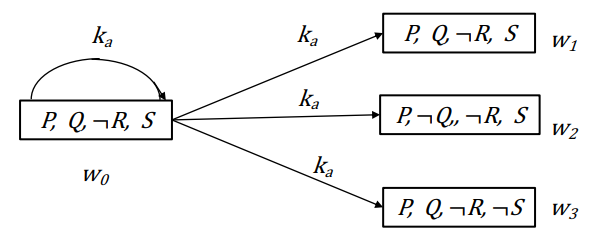
\includegraphics[scale=0.5]{15.png}
\end{center}
The accessibility relation also accounts for nested knowledge statements, also involving different agents. Knows($a$, Knows($b,P$)) holds in $w_0$ since Knows($b, P$) holds in $w_0,w_1,w_2$ and $w_3$ accessible to $a$.
\begin{center}
	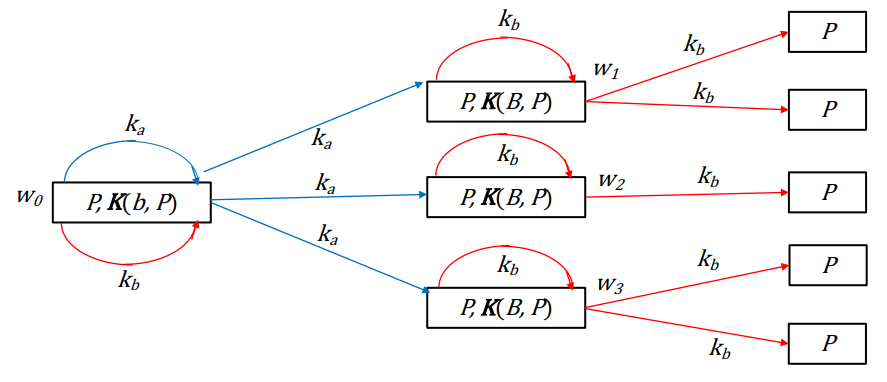
\includegraphics[scale=0.5]{16.png}
\end{center}
\subparagraph{Properties and axioms for knowledge} Many of the properties that we desire for the knowledge can be achieved by imposing constraints to the accessibility relation.
\begin{enumerate}
	\item Agents should be able to reason with the knowledge they have\\
	Knows$(a, \alpha\Rightarrow\beta)$ $\Rightarrow$ (Knows$(a,\alpha)$ $\Rightarrow$ Knows($a,\beta$)), \textbf{distribution axiom}\\
	Implicit in possible worlds semantics
	\item Agents cannot have false knowledge\\
	Knows($a,\alpha$) $\Rightarrow$ $\alpha$, \textbf{knowledge axiom}\\
	Satisfied if the accessibility relation is \textbf{reflexive}, i.e. Knows($a,w,w$) for every $a$ and every $w$. An implication is that $\neg$Knows($a$, false)\\
	Moreover, it implies that the relation is also \textbf{serial}, i.e. there's at least a worlds accessible from $w$.
	\item It's reasonable to assume that if an agent knows something, then it knows that it knows\\
	Knows($a,\alpha$) $\Rightarrow$ Knows($a$, Knows($a,\alpha$)), \textbf{positive introspection}\\
	The accessibility relation must be \textbf{transitive}, i.e. Knows($a,w_1,w_2$) $\wedge$ Knows($a,w_2,w_3$) $\Rightarrow$ Knows($a,w_1,w_3$)
	\item In some axiomatization we also assume that if an agent doesn't know something, then it knows that it doesn't know\\
	$\neg$Knows($a,\alpha$) $\Rightarrow$ Knows($a$, $\neg$Knows($a,\alpha$)), \textbf{negative introspection}\\
	The accessibility relation must be \textbf{euclidean}, i.e.Knows($a,w_1,w_2$) $\wedge$ Knows($a,w_1,w_3$) $\Rightarrow$ Knows($a,w_2,w_3$)
	\item It's also intrinsic in possible worlds semantic that an agent knows all the logical theorems, including the ones characterizing knowledge\\
	From $\vdash\alpha$ infer Knows$(a,\alpha)$, \textbf{epistemic necessitation rule}
	\item From the first and fifth properties, we can also get the rules
	\begin{list}{}{}
		\item From $\alpha\vdash\beta$ and Knows($a,\alpha$) infer Knows($a,\beta$)
		\item From $\vdash\alpha\Rightarrow\beta$ infer Knows($a,\alpha$) $\Rightarrow$ Knows($a,\beta$)
	\end{list}
	This is called \textbf{logical omniscience}, is considered problematic: we are assuming unbounded reasoning capabilities. As a corollary of logical omniscience we have Knows$(a,\alpha\wedge\beta)$ $\equiv$ Knows$(a,\alpha)$ $\wedge$ Knows($a,\beta$) (Knows distribution over $\wedge$)\\
	It's however not the case that Knows$(a,\alpha\vee\beta)$ $\equiv$ Knows$(a,\alpha)$ $\vee$ Knows($a,\beta$)
\end{enumerate}
Modal epistemic logics are obtained with various combination of axioms 1-4 plus inference rule 5:
\begin{list}{}{}
	\item System K: axiom 1
	\item System T: axioms 1-2
	\item Logic S4: axioms 1-3
	\item Logic S5: axioms 1-4 (perfect reasoner)
\end{list}
Not any combination is possible since the properties of accessibility are interdependent, for example: reflexive implies serial, a reflexive and euclidean relation is also transitive (axioms 2 and 4 impliy 3), \ldots
\subparagraph{Properties and axioms for beliefs} Since an agent can hold wrong beliefs, the knowledge axiom is not appropriate. Instead, we include as an axiom the following: $neg$Believe($a$, False), \textbf{lack of contradictions}.\\The distribution axiom and the necessitation rule are controversial, since an agent cannot realistically believe all the logical consequences of its beliefs but only those that he is able to derive (\textbf{limited/bounded rationality}).
\begin{list}{}{}
	\item Believe($a,\alpha$) $\Rightarrow$ Believe($a$, Believe($a,\alpha$)), \textbf{positive introspection}
	\item Believe($a,\alpha$) $\Rightarrow$ Believe($a$, Believe($a,\alpha$)) is also reasonable
\end{list}
Negative introspection is problematic, while the following special case of the knowledge axioms is safe: Believe($a$, Believe($a,\alpha$)) $\Rightarrow$ Believe($a,\alpha$)\ldots
\subsection{Autoepistemic Logic}
At the intersection between Modal Logics for Beliefs and Nonmonotonic Logic.\\
$\frac{\alpha : \beta}{\gamma}$, in default logic, is read as "if $\alpha$ and \textit{it is consistent to believe $\beta$} then $\gamma$"\\
A different approach to nonmonotoninc reasoning is to model "\textit{it is consistent to believe $\beta$}" as the lack of belief in $\neg\beta$ with a suitable logic for belief.
\paragraph{Autoepistemic Logic} It uses a belief operator $B$. $B\alpha$ stands for "$\alpha$ is believed to be true". The $B$ operator could be used to represent defaults, for example:
\begin{list}{}{}
	\item $\forall\:x$ Bird$(x) \wedge\neg B\neg$Flies$(x)\Rightarrow$ Flies$(x)$\\
	Any bird not believed to be unable to fly, does fly.
\end{list}
Note that $B\neg$Flies$(x)$ is different from $\neg$Flies$(x)$\\\\
Given a KB that contains sentences with the $B$ "autoepistemic" operator, what is a reasonable set of beliefs $E$ to hold? Minimal properties of a set of beliefs $E$ to be considered stable:
\begin{list}{}{}
	\item Closure under entailment: if $E\vDash\alpha$ then $\alpha\in E$
	\item Positive introspection: if $\alpha\in E$ then $B\alpha\in E$
	\item Negative introspection: if $\alpha\not\in E$ then $\neg B\alpha\in E$
\end{list}
This leads to a the definition of a stable expansion of a KB (minimal set satisfying all three properties)
\paragraph{Stable Expansion of the KB} A set $E$ is a stable expansion of KB $\Leftrightarrow\:\forall$ sentence $\pi$ we have
$$\pi\in E \Leftrightarrow KB\cup\{B\alpha\:|\:\alpha\in E\}\cup\{\neg B\alpha\:|\:\alpha\not\in E\}\vDash\pi$$
with $\{B\alpha\:|\:\alpha\in E\}\cup\{\neg B\alpha\:|\:\alpha\not\in E\}$ being the set of assumed beliefs. The \textbf{implicit beliefs} $E$ are those sentences entailed by KB plus the assumptions deriving from positive and negative introspection.
%KRR-5.pdf
\subsection{Graph representation and structured representation}
\subsubsection{Psychological-linguistic approach to KR\&R}
\paragraph{Logical Approach} Suitable to model rational reasoning: extension to model commonsense reasoning (frame problem, nonmonotonic reasoning, propositional attitudes\ldots), FOL contradictions to control computational complexity of reasoning (description logics, logic programming\ldots)
\paragraph{Cognitive-Linguistic Approach} More concerned with understanding the mechanisms for knowledge acquisition, representation and use in human minds. Synergies with other fields, such as cognitive psychology and linguistics.
\paragraph{Associationist theories of KR} In logic systems, symbolic expressions are modular and are syntactically transformed without paying attention to the symbols used or to their "meaning". The symbol themselves are arbitrary: it's all a matter of writing axioms to restrict interpretations.\\
Associationist theories are instead concerned with the connection among symbols, and the meaning that emerges from these connections. The idea is that the meaning of a symbol emerges as a result of the connections to other symbols. The connections are shaped by experience.
\subsubsection{Semantic Networks}
\paragraph{Semantic Memory} The problems is how the meaning of the symbols/words is acquired, represented and used. The memory itself is distinguished in:
\begin{list}{}{}
	\item \textbf{Episodic memory}: specific facts and events
	\item \textbf{Semantic memory}: abstract and general knowledge
\end{list}
\textbf{Semantic Networks} is a graphical model proposed for semantic memory, with two kinds of knowledge:
\begin{list}{}{}
	\item \textbf{Concepts}: semantic counterpart of words, represented as nodes
	\item \textbf{Propositions}: relations among concepts, represented as labelled arcs
\end{list}
No account for dynamic aspects of memory and learning. Other models are: distributional models (example: word embeddings) or connectionist models for learning.
\paragraph{Essence of semantic networks} It's a large family of graphical representation schemes. A semantic network is a graph where: labeled \textbf{nodes} correspond to \textbf{concepts} and labeled and directed \textbf{arcs} correspond to \textbf{binary relations between concepts}.\\
Node come in two flavors: \textbf{generic concepts}, corresponding to categories/classes, and \textbf{individual concepts} corresponding to individuals.\\
Two special kind of links are always present, with different names: \textbf{IS-A} (sublcass, between two generic concepts) and \textbf{Inst-Of} (member of, between and individual concept and a class).\\
An example:
\begin{center}
	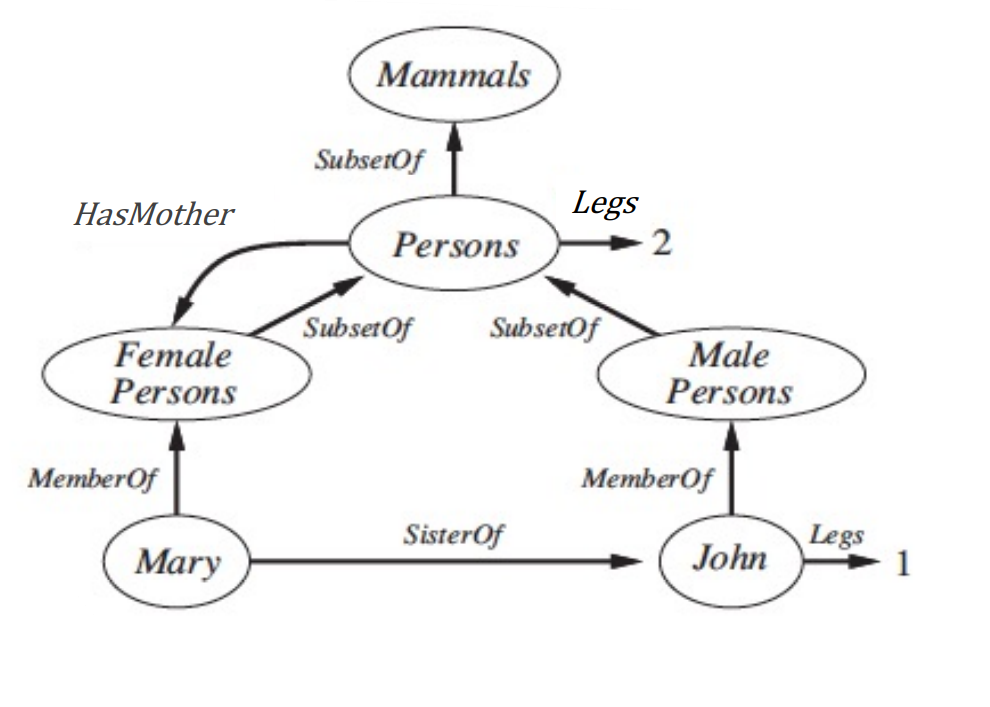
\includegraphics[scale=0.5]{17.png}
\end{center}
\subparagraph{Inheritance} Implemented as link traversal: find the first occurrence of the property that you seek.
\subparagraph{Logic accounts} We may look at semantic networks as a convenient implementation for a part of FOL: representation and mechanism at the symbol level rather than at the knowledge level
\begin{list}{}{}
	\item $A \begin{array}{c}
	\hbox{IS-A}\\\longrightarrow
	\end{array} B$\\
	$\forall\:x\:\:A(x)\Rightarrow B(x)$\\
	All members of class $A$ are also members of class $B$
	\item $a \begin{array}{c}
	\hbox{Inst-Of}\\\longrightarrow
	\end{array} B$\\
	$B(a)$\\
	$a$ belongs to class $B$
	\item $A \begin{array}{c}
	\hbox{R}\\\longrightarrow
	\end{array} b$\\
	$\forall\:x\:\:x\in A\Rightarrow R(x,b)$\\
	All members of class $A$ are in relation $R$ with $b$
	\item $A \begin{array}{c}
	\hbox{R}\\\longrightarrow
	\end{array} B$\\
	$\forall\:x\:\:x\in A\Rightarrow \exists\:y\:\:y\in B \wedge R(x,y)$\\
	For all members of class $A$, there is a $R$-related element in $B$
\end{list}
An example of "Shankar flew from New York to New Deli yesterday"
\begin{center}
	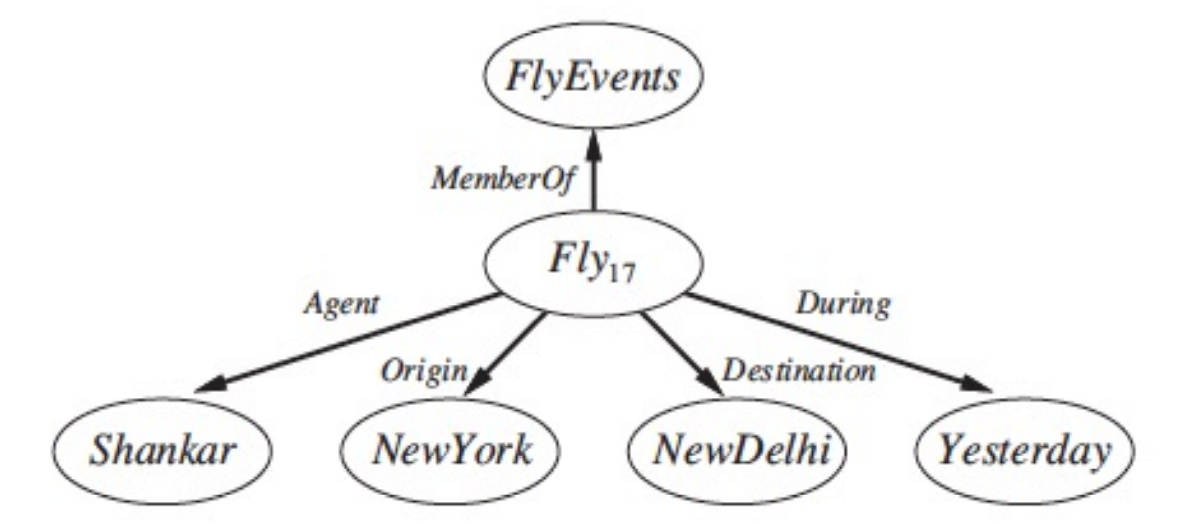
\includegraphics[scale=0.5]{18.png}
\end{center}
\subparagraph{Limited expressive power} Even if they can express $n$-ary predicates like in the example above, semantic networks do not have the same expressive power of FOL: Existential, $\vee$, $\Rightarrow$,\ldots are not expressible or are expressible only in special cases. Not necessarily a bad case, since it suggests that a subset of FOL with interesting computational properties, explored in description logics.\\
More expressive assertional networks ere proposed in the past. A well-known example in AI are Pierces's Existential Graphs, which inspired Sowa's Conceptual Graphs: they candidate as an intermediate schema for representing natural language.
\subsection{Object Oriented Representations and Frames}
It's very natural to think of knowledge not as a flat collection of sentences, but rather as a structured and organized collection in terms of the objects the knowledge is about. Complex objects have attributes, part constrained in various ways. Objects might have a behavior that is better expressed as procedures (like in OOP).\\
\subsubsection{Frames} Nothing to do with frame problems, proposed by Minsky in 1975: idea of using a structured representation of objects.\\
Knowledge is organized in complex mental structures called \textbf{frames}. When one encounters a new situation (or makes a substantial change in one's view of the present problem) one selects from memory a structure called a frame: this is a remembered framework to be adapted to fit reality by changing details as necessary.\\
A \textbf{frame} is a \textbf{data structure for representing a stereotypical object or situation}. There are two types:
\begin{list}{}{}
	\item \textbf{Individual frames}, used to represent single objects\\
	Is a collection of slot-filler pairs:
	\begin{verbatim}
		(Frame-Name
			<slot1 filler1>
			<slot2 filler2>
			...)
	\end{verbatim}
	Fillers can be: values (usually default values), constraints on values, names of other individual frames, the special slot INSTANCE-OF. Example:
	\begin{verbatim}
	(toronto
		<:INSTANCE-OF CanadianCity>
		<:Province ontario>
		<:Population 4.5M>
		...)
	\end{verbatim}
	\item \textbf{Generic frames}, used to represent categories or classes of objects.\\
	Similar to individual frames, where fillers can be: the special slot IS-A or procedures (IF-ADDED, activated when the slot receives a value, or IF-NEEDED, activated when the value is requested)\\
	These procedures are calles \textbf{procedural attachments} or demons. An example:
	\begin{verbatim}
	(CanadianCity
		<:IS-A City>
		<:Province CanadianProvince>
		<:Country Canada>
		...)
		
	(Lecture
		<:DayOfWeek WeekDay>
		<:Date [IF-ADDED ComputeDayOfWeek]>
		...)
		
	(Table
		<:Clearance [IF-NEEDED ComputeClearanceFromLegs]>
		...)
	\end{verbatim}
\end{list}
The INSTANCE-OF and IS-A slots organize frames in frame systems: they have the special role of activating inheritance of properties and procedures. In frames, all values are understood as default values, which can be overwritten.
\paragraph{Reasoning with frames} Attached procedure provide a flexible, organized framework for computations: reasoning has a procedural flavor.\\
A basic reasoning loop in a frame system has three steps:
\begin{list}{}{}
	\item \textbf{Recognition}: a new object or situation is recognized as instance of a generic frame
	\item \textbf{Inheritance}: any slot fillers that are not provided explicitly but can be inherited by the new frame instance are inherited
	\item \textbf{Demons}: for each slot with a filler, any inherited IF-ADDED procedure is run, possibly causing new slots to be filled, or new frames to be instantiated, until the system stabilizes.\\
	Then the cycle repeats.
\end{list}
When the filler of a slot is requested:
\begin{list}{}{}
	\item If there's a value stored, it's returned
	\item Otherwise, any inherited IF-NEEDED procedure is run to compute the filler for the slot. This may cause other slots to be filled, or new frames to be instantiated.
\end{list}
\paragraph{Frames and OOP} Frame-based representation languages and OOP systems were developed at the same time. They look similar and certainly one could implement a frame system in OOP. The \textbf{important difference} is that frame systems tend to work in a cycle:
\begin{list}{}{}
	\item Instantiate a frame and declare some slot fillers
	\item Inherit values from more general frames
	\item Trigger appropriate forward-chaining procedures
	\item When the system is quiescent, stop and wait for the next input
\end{list}
The design can control the amount of "forward" reasoning that should be done (in a data-directed fashion) or "backward" (in a goal-directed fashion)
%KRR-6.pdf
\subsection{Description Logics} 
\paragraph{Categories and Objects} Most of the reasoning takes place at the level of categories rather than on individuals. If we organize knowledge in categories and subcategories (in a hierarchy), it's enough to classify an object according to its perceived properties, in order to infer properties of the categories to which it belongs. \textbf{Inheritance} is the common form of inheritance, which exploits structures. \textbf{Ontologies} will play a crucial role, providing a source of shared and precisely defined terms that can be used in metadata of digital objects and real-world objects.
\paragraph{Domain ontologies} The formalization of the ideas coming from semantic networks and frames resulted in \textbf{specialized logics}. These logics, called \textbf{terminological logics} and later \textbf{description logics}, find an important application in describing "domain ontologies" and represent the theoretical foundations for adding reasoning capabilities to the \textbf{semantic web}. \textbf{Ontology} is a \textbf{formal model of an application domain}, a \textbf{conceptualization}.\\
the \textbf{semantic web} is the vision to gradually develop alongside the "syntactic web" (or web of documents), for communication among people, a "semantic web" (or web of data), form communication among the machines. It's a huge distributed network of linked data, which can be used by programs as well, provided their semantics is shared and made clear (role of formal ontologies).
\begin{center}
	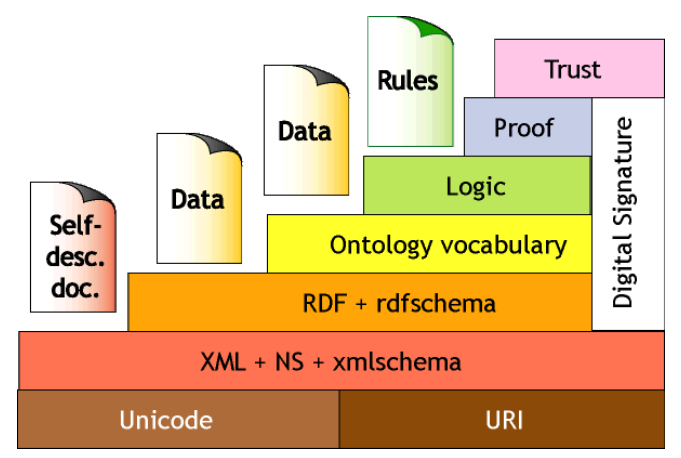
\includegraphics[scale=0.5]{19.png}
\end{center}
\paragraph{Description logics} Can be seen as:
\begin{list}{}{}
	\item Logical counterparts of network knowledge representation schemas, frames and semantic networks.\\
	In this formalization effort, defaults and exceptions are abandoned. The ideas and terminology (concept, roles, inheritance) are very similar (to KLOne in particular)
	\item Contractions of FOL, investigated to obtain better computational properties. Attention to computational complexity and decidability of the inference mechanisms.
\end{list}
An example: "paper3 has exactly two authors"
\begin{list}{}{}
	\item (\textbf{and} Paper (\textbf{atmost} 2 hasAuthor) (\textbf{atleast} 2 hasAuthor)) [paper3]
	\item We'll use the alternative, \textbf{mathematical notation}\\
	paper3: Paper $\sqcap$ ($\leq$ 2 hasAuthor) $\sqcap$ ($\geq$ 2 hasAuthor)
	\item The corresponding in FOL is\\
	Paper(paper3) $\wedge$ $\exists\:x$ hasAuthor(paper3, $x$) $\wedge$ $\exists\:y$ hasAuthor(paper3, $y$) $\wedge$ $x\neq y$ $\wedge$ hasAuthor(paper3, $z$) $\Rightarrow (z = x) \vee (z = y)$
\end{list}
\paragraph{Concepts, roles, individuals} Each DL is characterized by operators for the construction of terms.\\
\textbf{Terms} (description) are of three types:
\begin{list}{}{}
	\item \textbf{Concepts}, corresponding to unary relations, with operators for the construction of complex concepts: and ($\sqcap$), or ($\sqcup$), not ($\neg$), all ($\forall$), some ($\exists$), atleast ($\geq n$), atmost ($\leq n$), \ldots
	\item \textbf{Roles}, corresponding to binary relations, possibily together with operators for construction of complex roles
	\item \textbf{Individuals}, only used in assertions
\end{list}
\textbf{Assertions} are kept separate and can be of two types:
\begin{list}{}{}
	\item $i:C$, where $i$ is an individual and $C$ a concept
	\item $(i,j):R$, where $i,j$ are individuals and $R$ a role
\end{list}
%TODO KRR-6.pdf p.11
\section{Reasoning Under Uncertainty}
\subsection{Quantifying Uncertainty}
Agents are inevitable forced to reason and make decisions based on incomplete information. They need a way to handle uncertainty deriving from:
\begin{list}{}{}
	\item \textbf{Uncertainty in sensors}: partial observability
	\item \textbf{Uncertainty in actions}: nondeterministic actions
\end{list}
A partial answer would be to consider a set of possible worlds (a \textbf{belief set}, which are considered possible by the agent), but planning by anticipating all possible contingencies can be really complex. Moreover, if no plan guarantees the achievement of the goal but the agent still needs to act, how can he evaluate the relative merits of alternative plans? \textbf{Probability theory} offers a clean way to quantify uncertainty (common sense reduced to calculus).\\
With a logical approach, it is difficult to anticipate everything "that could go wrong" (\textbf{quantification problem}). The rational decision depends on both the \textbf{relative importance} of the various goals and the \textbf{likelihood} that they will be achieved. When there are conflicting goals, the agent may express \textbf{preferences} by the means of a utility function. Utilities are combined with probabilities in the general theory of rational decisions called \textbf{decision theory}.\\
An agent is rational $\Leftrightarrow$ it chooses \textbf{the action that yields the maximum expected utility, averaged over all the possible outcomes of the action}. This is called the principle of \textbf{Maximum Expected Utility} (\textbf{MEU}).
\paragraph{Probability Theory} Logic and probability theory both talk about a world made of propositions which are \textit{true} or \textit{false}. They share the \textbf{ontological commitment}.\\
What's different is the \textbf{epistemological commitment}: a logical agent believes each sentence to be true or false or has no opinion, whereas a probabilistic agent may have a numerical \textbf{degree of belief} between 0 (certainly false) and 1 (certainly true). The uncertainty is not in the world, but in the beliefs of the agent (\textbf{state of knowledge}). If the knowledge about the world changes (we learn more information) the probability changes, but there is no contradiction.
\subparagraph{Probabilities} In AI terms: probabilistic assertions are assertions about possible worlds stating how probable a world is. The set of possible world is the \textbf{sample space} $\Omega$: they are mutually exclusive and exhaustive. For example, the 36 possible outcomes of rolling two dices.\\
A fully specified probability model associates a probability $P\in R, 0\leq P \leq 1$ to each possible world $\omega\in\Omega$.\\
The \textbf{basic axiom of probability} is $$0\leq P(\omega)\leq 1\:\:\forall\:\omega\in\Omega\hbox{ and }\sum_{\omega\in\Omega} P(\omega) = 1$$
Usually we deal with a subset of possible worlds (\textbf{events}) which can be described by an expression (\textbf{proposition}) in a formal language. The \textbf{events} are the possible worlds where the proposition holds. Also for any event $\Phi$ we have that $P(\Phi) = \sum_{\omega\in\Phi} P(\omega)$
\subparagraph{Conditional probabilities} Often we have evidence that restrict the number of possible worlds, conditioning the probability of an event. These probabilities are called \textbf{conditional}/posterior probabilities: $P(a\:|\:b) = \frac{P(a,b)}{P(b)}$ with $P(b) > 0$. Note that $P(a,b)=P(a\:|\:b)P(b)$
\paragraph{Probability distribution} A full specification of the probability for all values of a variable $X$ is a \textbf{probability distribution}.
\begin{list}{}{}
	\item \textbf{Discrete} For example
	\begin{list}{}{}
		\item $P($Weather $=$ sunny$)=0.6$
		\item $P($Weather $=$ rain$)=0.1$
		\item $P($Weather $=$ cloudy$)=0.29$
		\item $P($Weather $=$ snow$)=0.01$
	\end{list}
	can be expressed with a vector $P$ to represent the distribution: $P($Weather$) = \langle 0.6,0.1,0.29,0.01\rangle$\\
	$P(X\:|\:Y)$ is the table of values $P(X=x_1\:|\:Y=y_i)$ one value for each pair $i,j$.
	\item \textbf{Continuous} For continuous variables we can define the probability that a random variable takes some value $x$ as a function of $x$, called \textbf{probability density function} or \textbf{PDF}.\\
	If $f$ is the density function, then $P(a\leq x\leq b) = \int_a^b f(x)\:dx$, $\int_{-\infty}^{+\infty} f(x)\:dx = 1$ for $f(x)\geq 0$
\end{list}
A \textbf{joint probability distribution} is a distribution over a set of variables.
\paragraph{Semantics} A possible world is defined to be an assignment of values to all the random variables under consideration. It follows that possible worlds are mutually exclusive and exhaustive.\\
The truth of a complex proposition in a world can be determined using the same recursive definition of truth used for formulas in PROP.\\
If we have a joint probability distribution of all the variables (\textbf{full joint probability distribution}), then we can perform an inference. Given that
\begin{list}{}{}
	\item A proposition identifies a set of possible worlds
	\item An entry in the table gives the probability of a possible world
	\item For any event $\Phi, P(\Phi) = \sum_{\omega\in\Omega} P(\omega)$
\end{list}
we can compute the probability of any proposition by taking the sum of the probabilities of the relevant possible worlds in the distribution.
\paragraph{Properties of discrete variables} Known as \textbf{Kolmogorov's axioms}:
\begin{list}{}{}
	\item $0\leq P(\omega)\leq 1\:\:\forall\:\omega\in\Omega$ and $\sum_{\omega\in\Omega}P(\omega)=1$
	\item For any proposition $\Phi,P(\Phi)=\sum_{\omega\in\Omega}P(\omega)$
	\item $P(\neg a)=1-P(a)$
	\item $P(a\vee b) = P(a) + P(b) - P(a\wedge b)$ (\textbf{inclusion-exclusion principle})
\end{list}
\paragraph{Plausibility} If an agent holds an inconsistent set of beliefs, the if it bets according to this set of beliefs against another agent, then the other agent can devis a strategy to make it always lose money. De Finetti's theorem implies that no rational agent can have beliefs that violate the axioms of probability.
\subsubsection{Probabilistic Inference} Assuming we have a full joint distribution as the knowledge base, we will use the axioms of probability and show how to:
\begin{list}{}{}
	\item Compute \textbf{marginals}, prior probability of a single variable
	\item Compute the probability of complex propositions ($\wedge,\vee,\neg$)
	\item Compute the \textbf{posterior probability} for a proposition given observed evidence
\end{list}
\paragraph{Computing marginals} Probability of a variable from the full joint distribution. Given a joint distribution $P(X,Y)$ over variables $X$ and $Y$, the distribution of the single variable $X$ is given by $$P(X) = \sum_{y\in dom(Y)}P(X,y) = \sum_y P(X,y)$$
Also called \textbf{marginalization} or \textbf{summing out}. In general, if $Y$ and $Z$ are sets of variables such that $Y\cup Z$ are all the variables in the full joint distribution, then $P(Y) = \sum_{z\in Z}P(Y,z)$
\subparagraph{Conditioning} Variant of the marginalization, involving conditional probabilities instead of joint probability: can be obtained from the previous using the product rule $$P(Y) = \sum_{z\in Z} P(Y\:|\:z)P(z)$$
\paragraph{General inference procedure} If the query involves a single variable $X$, $e$ is the list of the observed values (the evidence) and $Y$ the rest of unobserved variables, then $$P(X\:|\:e) = \alpha P(X,e) = \alpha\sum_y P(X,e,y)$$
However it's intractable due to the complexity of the joint distribution table: with $n$ boolean variables, it requires an input table of size $O(2^n)$ and $O(2^n)$ time to process.
\paragraph{Independence} Independence of propositions $a,b$: $P(a\:|\:b) = P(a)$, $P(b\:|\:a)=P(b)$, $P(a,b)=P(a)P(b)$\\
Independence of variables $X,Y$: $P(X\:|\:Y) = P(X)$, $P(Y\:|\:X)=P(Y)$, $P(X,Y)=P(X)P(Y)$\\
Independence assumptions can reduce the size of the representation and the complexity of the inference problems. A notation for the independence $X\perp Y$.
\paragraph{Bayes theorem} $$P(Y\:|\:X) = \frac{P(X\:|\:Y)P(Y)}{P(X)}$$
This tells us how to update the agent's believes in hypothesis $h$ as new evidence $e$ arrives, given the background knowledge $k$ $$P(h\:|\:e,k)=\frac{P(e\:|\:h,k)P(h\:|\:k)}{P(e\:|\:k)}$$
$X$ and $Y$ are \textbf{conditionally independent given $Z$} when $P(X,Y\:|\:Z)=P(X\:|\:Z)P(Y\:|\:Z)$. Alternatively, when \begin{list}{}{}
	\item $P(X\:|\:Y,Z) = P(X\:|\:Z)$
	\item $P(Y\:|\:X,Z) = P(Y\:|\:Z)$
\end{list}
\paragraph{Naive Bayes model} $P($Cause, Effect$_1$, \ldots, Effect$_n) = P($Cause$)\prod_i P($Effect$_i\:|\:$Cause$)$
\subsection{Probabilistic Reasoning} 
\paragraph{Bayesian Networks} Also called \textbf{belief networks}: graphs for representing dependencies among variables. The network makes specific conditional dependencies: the intuitive meaning of an arc from $X$ to $Y$ is typically that $X$ has a direct influence on $Y$.\\
Bayesian Networks are \textbf{directed acyclic graphs} (DAG) so defined:
\begin{list}{}{}
	\item Each node corresponds to a random variable, which may be discrete or continuous.
	\item Directed links or arcs connect pairs of nodes. If there's an arc from node $X$ to node $Y$, $X$ is said to be a parent of $Y$: Parents($Y$) is the set of variables directly influencing $Y$.
	\item Each node $X$ has an associated \textbf{conditional probability distribution table} $P(X\:|$ Parents$(X))$ that quantifies the effect of the parents on the node.
\end{list}
It's easier to decide what direct influences exist in the domain than actually specifying the probability themselves.
\paragraph{Cavity \& Weather example}
\begin{center}
\begin{tikzpicture}[node distance={25mm}, main/.style = {draw, circle}] 
\node[main] (1) {Weather}; 
\node[main] (2) [right of=1,yshift = -1cm] {Cavity}; 
\node[main] (3) [below left of=2] {Toothache}; 
\node[main] (4) [below right of=2] {Catch}; 
\draw[->] (2) -- (3);
\draw[->] (2) -- (4);
\end{tikzpicture} 
\end{center}
Weather is independent from the other variables, and Toothache and Catch are \textbf{conditionally dependent} given Cavity. The \textbf{lack of an arc between two variables} is interpreted as \textbf{independence}.
\paragraph{Alarm example} \textit{The burglary alarm goes off very likely on burglary and occasionally on earthquakes. John and Mary are neighbors who agreed to call when the alarm goes off. Their reliability is different\ldots}
\begin{center}
\begin{tikzpicture}[node distance={25mm}, main/.style = {draw, circle}] 
\node[main] (1) {Burglary}; 
\node (6) [left of=1] {\begin{tabular}{|c|}
\hline P(B)\\\hline.001\\\hline
\end{tabular}};
\node[main] (2) [right of=1] {Earthquake};
\node (7) [right of=2] {\begin{tabular}{|c|}
\hline P(E)\\\hline.002\\\hline
\end{tabular}};
\node[main] (3) [below left of=2,yshift = -1cm] {Alarm}; 
\node (8) [right of=3] {\begin{tabular}{|c|c|c|}
\hline B&E&P(A)\\
\hline t&t&.95\\
t&f&.94\\
f&t&.29\\
f&f&.001\\
\hline
\end{tabular}};
\node[main] (4) [below right of=3,yshift = -1cm] {MaryCalls};
\node (9) [right of=4] {\begin{tabular}{|c|c|}
\hline A&P(M)\\
\hline t&.70\\
f&.01\\
\hline
\end{tabular}};
\node[main] (5) [below left of=3,yshift = -1cm] {JohnCalls}; 
\node (10) [left of=5] {\begin{tabular}{|c|c|}
\hline A&P(J)\\
\hline t&.90\\
f&.05\\
\hline
\end{tabular}};
\draw[->] (1) -- (3);
\draw[->] (2) -- (3);
\draw[->] (3) -- (4);
\draw[->] (3) -- (5);
\end{tikzpicture} 
\end{center}
The tables are called \textbf{Condition Probability Tables}.
\subsubsection{Semantic of Bayesian Networks}
Two alternative and equivalent ways to look at the semantic of Bayesian Networks:
\begin{list}{}{}
	\item Distributed representation of the full joint probability distribution\\
	Suggests a metodology for constructing networks
	\item Encoding of a collection of conditional independence statements\\
	Helps in designing inference procedures
\end{list}
\paragraph{Representation of the full joint distribution} A joint probability distribution can be expressed in terms of conditional probabilities
\begin{list}{}{}
	\item $P(x_1,\ldots,x_n) = P(x_n\:|\:x_{n-1},\ldots,x_1)\cdot P(x_{n-1},\ldots,x_1)$, product rule
\end{list}
And by iterating the process we get the \textbf{chain-rule}
\begin{list}{}{}
	\item $P(x_1,\ldots,x_n) = P(x_n\:|\:x_{n-1},\ldots,x_1)P(x_{n-1}\:|\:x_{n-2},\ldots,x_1)\ldots P(x_2\:|\:x_1)P(x_1) = \prod_{i=1}^n P(x_i\:|\:x_{i-1},\ldots,x_1)$
\end{list}
So we assumed an order of the variables, we computed posterior probabilities of each variable, given all previous variables and we took the product of these posteriors.
\subparagraph{Representing the joint probability distribution} Given that $P(x_1,\ldots,x_n) = \prod_{i=1}^n P(x_i\:|\:x_{i-1},\ldots,x_1)$ and assuming\begin{list}{}{}
	\item Each variable appears after its parents in the ordering, meaning Parents$(X_i) \subseteq \{X_{i-1},\ldots,X_1\}$
	\item We simplify the computation by conditioning the computation only to values of the parent variable (assuming the others are independent)
	\item The numbers in the Condition Probability Tables are actually conditional probabilities.
\end{list}
Each entry in the joint distribution can be computed as the product of the appropriate entries in the conditional probability tables (CPTs) in the Bayesian network. We get the \textbf{simplified rule} for computing joint distributions: $$P(x_1,\ldots,x_n) = \prod_{i=1}^n P(x_i\:|\:\hbox{Parents}(x_i))$$
Given the Alarm example and the ordering $(J,M,A,B,E)$ we can compute, by the chain rule \begin{list}{}{}
	\item $P(j,m,a,\neg b, \neg e) = P(j\:|\:m,a,\neg b, \neg e)P(m\:|\:a,\neg b, \neg e)P(a\:|\:\neg b, \neg e)P(\neg b\:|\:\neg e)P(\neg e)$
\end{list}
And taking into account only direct dependencies, we can simplify as \begin{list}{}{}
	\item $P(j,m,a,\neg b, \neg e) = P(j\:|\:\cancel{m},a,\cancel{\neg b, \neg e})P(m\:|\:a,\cancel{\neg b, \neg e})P(a\:|\:\neg b, \neg e)P(\neg b\:|\:\cancel{\neg e})P(\neg e)$
\end{list}
And using the probability values from the CPTs we get $P(j\:|\:a)P(m\:|\:a)P(a\:|\:\neg b,\neg e)P(\neg b)P(\neg e) = 0.9\cdot0.7\cdot0.001\cdot0.999\cdot0.998=0.000628$
\subparagraph{Procedure for building the network}
\begin{list}{}{}
	\item Nodes: determine the set of variables required to model the domain, and order them $\{X_1,\ldots,X_n\}$\\
	\textbf{Ordering influences the result}: the resulting network will be more compact if the variables are ordered such that causes precedes effects.
	\item Liks: for $i=1$ to $n$ do
	\begin{list}{}{}
		\item Choose, from $X_1,\ldots,X_{i-1}$ a minimal set of parents for $X_i$ such that the equation $P(X_i\:|\:X_{i-1},\ldots,X_1) = P(X_i\:|\:$Parents$(X_i))$ is satisfied
		\item For each parent insert an arc from the parent to $X_i$
		\item CPTs: write down the conditional probability table $P(X_i\:|\:$Parents$(X_i))$
	\end{list}
\end{list}
Note that the parents of $X_i$ should contain all the nodes that \textbf{directly} influence $X_i$. Also the network is a DAG by construction and contains no redundant probability values.\\
In \textbf{locally structured systems} each subcomponent interacts directly only with a bounded number of other components. They are usually associated with linear rather than exponential growth in complexity. In the case of Bayesian networks, it is reasonable to suppose that in most domains each random variable is directly influenced by at most $k$ others, for some constant $k$.\\
If we assume $n$ boolean variables, then each conditional probability table will have at most $2^k$ numbers, and the complete network can be specified by $n\cdot2^k$ numbers. In contrast, the joint distribution contains $2^n$ numbers.
\paragraph{Conditional Independence} We can also extract the independence assumptions encoded in the graph to do inference. The topological semantics specifies that each variable is conditionally independent of its non-descendants, given its parents. In our example, the network tells us that JohnCalls is independent of Burglary, Earthquake and MaryCalls given the value of Alarm. This autorizes the following semplification $P(J,B,E,M\:|\:A)= P(J\:|\:A)P(M\:|\:A)P(B)P(E)$\\
A node is conditionally independent of all other nodes in the network given its parents, children and children's parents.
\paragraph{Efficient construction of CPTs} Often, the relationship between a node and its parent follows a canonical distribution and the construction of the CPTs can be simplified. Two examples:
\begin{list}{}{}
	\item \textbf{Deterministic Nodes}: nodes whose value is specified exactly by the values of their parents. For example, Price$_1$,\ldots,Price$_k$ (the parents) determine $min$(Price$_1$,\ldots,Price$_k$) (the best price)
	\item \textbf{Noisy-OR Relations}: a generalization of the logical OR. We can specify inibiting factors, so that A$\vee$B$\Leftrightarrow$C but not always. The probability of $\neg$C is the product of the inibition probabilities $q$ for each parent that is true. It is $1$ when none of the causes are true. $P(x_i\:|\:$Parents$(X_i)) = 1-\prod_{\{j\:|\:X_j=\hbox{true}\}}q_j$
\end{list}
\paragraph{Continuous variables} One possible way to handle them is to avoid them and use discrete intervals. For example, temperature into three intervals: $<0$°C, $[0,100]$°C, $>100$°C.\\
The most common solution is to define standard families of probability density function that are specified by a finite number of parameters, for example a Gaussian (normal) distribution $N(\mu,\sigma^2)(x)$ with parameters the mean $\mu$ and the variance $\sigma^2$.\\
A network with both discrete and continuous variables is called hybrid Bayesian network.
\subsubsection{Exact inference in Bayesian Networks}
The basic task of probabilistic inference. Given:\begin{list}{}{}
	\item $X$: the query variable (assuming just one)
	\item $E$: the set of evidence variables $\{E_1,\ldots,E_m\}$
	\item $Y$: the set of unknown variables, i.e. the \textbf{hidden} non-evidence variables $\{Y_1,\ldots,Y_l\}$
	\item Thus $X = \{X\} \cup E \cup Y$
\end{list}
A typical query asks for the posterior probability distribution, given some evidence $P(X\:|\:e)$. In the alarm example, a query could be $P($Burglary$\:|\:$JohnCalls=true, MaryCalls=true$)$ with $E=\{$JohnCalls, MaryCalls$\}$ and $Y=\{$Earthquake, Alarm$\}$
\paragraph{Inference by enumeration} We defined a procedure for the task as $P(X\:|\:e)=\alpha P(X,e) = \alpha\sum_y P(X,e,y)$ with $\alpha$ being a normalizing factor.\\
The query can be answered using a Bayesian network by computing sums of products of conditional probabilities from the network. In the example: $P(B\:|\:j,m) = \alpha P(B,j,m) = \alpha\sum_e\sum_a P(B,j,m,e,a)$ summing over $y=\{E,A\}$\\
We can now use the CPTs for computing $P(B,j,m,e,a)$, i.e. the case of Burglary = true:
$$P(B\:|\:j,m) = \alpha\sum_e\sum_a P(B,j,m,e,a) = \alpha\sum_e\sum_aP(B)P(e)P(a\:|\:B,e)P(j\:|\:a)P(m\:|\:a)$$
And simplifying
$$P(B\:|\:j,m) = \alpha P(B)\sum_e P(e) \sum_a P(a\:|\:B,e)P(j\:|\:a)P(m\:|\:a)$$
The tree of computation is evaluated depth first, but the computation can be improved substantially by storing and reusing the results of repeated computations. The variable elimination algorithm proceeds right to left (bottom-up in the tree). Conditional probabilities are represented as factors, matrices resulting from conditional probabilities. In the example, it becomes
$$P(B\:|\:j,m) = \alpha f_1(B)\sum_e f_2(E) \sum_a f_3(A,B,E)f_4(A)f_5(A)$$
Given a variable and some evidence, a factor can be built by looking at the variable part of the CPT's in the network: \texttt{make-factor(var, e)}
\begin{list}{}{}
	\item \texttt{make-factor(M, [j,m]) = f5(A)} because $M$ only depends on $A$, $m$ is an evidence\\
	$f_5(A) = \langle P(m\:|\:a),P(m\:|\:\neg a)\rangle = \langle 0.7,0.01\rangle$
\end{list}
The pointwise product of two factors $f_1,f_2$ yields a new factor $f_3$ such that
\begin{list}{}{}
	\item variables are the union of the variables in $f_1$ and $f_2$
	\item elements are given by the product of the corresponding values in the two factors
\end{list}
So $f_1(A,B)\cdot f_2(B,C)$ gives $f_3(A,B,C)$\\\\
The ordering of variables can produce differences in efficiency. 
\paragraph{Complexity} Depends strongly on the structure of the network. Singly connected networks or polytrees are such that there is at most one undirected path between any two nodes (the Alarm network, for example). The time and space complexity in polytrees is linear in the size of network (the number of CPT entries). For multiply connected networks, variable elimination can have exponential time and space complexity in the worst case. In fact, inference in Bayesian networks includes as a special case propositional inference, which is NP-complete.
\subsection{Probabilistic Reasoning Over Time}
\paragraph{Reasoning in a changing world} So far, we've been reasoning in a static world. In an evolving world an agent needs:
\begin{list}{}{}
	\item A \textbf{belief state}: the states of the world which are possible
	\item A \textbf{transition model}: to predict how the world will evolve
	\item A \textbf{sensor model}: to update the belief state from perceptions
\end{list}
A changing world is modeled using a variable for each aspect of the world state \textbf{at each point in time} (\textbf{fluents}), and we use probabilities to quantify how likely a world is.\\
The transition and sensor model themselves may be uncertain:
\begin{list}{}{}
	\item The transition model gives the probability distribution of the variables at time $t$, given the state of the world at past times
	\item The sensor model describes the probability of each percept at time $t$, given the current state of the world
\end{list}
\subparagraph{The umbrella example} \textit{You are the security guard stationed at a secret underground installation. You want to know whether it's raining today, but your only access to the outside world occurs each morning when you see the director coming in with, or without, an umbrella.}
\paragraph{States and observations} We view the world as a series of snapshots, or \textbf{time slices}, each of which contains a set of random variables, some observable and some not.
\begin{list}{}{}
	\item $x_t$ will denote the set of \textbf{state variables}, unobservable (hidden) at time $t$
	\item $E_t = e_t$ will denote the set of observations (\textbf{evidence variables}) at time $t$, with $e_t$ being their values
\end{list}
The sequence starts at $t=0$ (state variables starts at 0, evidences at 1), and the distance between time slices is fixed.\\
With $a:b$ we will denote the sequence of integers from $a$ to $b$, inclusive, and with $x_{a:b}$ the set of variables from $x_a$ to $x_b$.\\
The umbrella world is represented by a sequence of evidence variables $E_t=\{U_t\}$ (whether the umbrella appears at time $t$) and state unobservable variables $x_t=\{R_t\}$ (it's raining):
\begin{list}{}{}
	\item State variables $R_0,R_1,R_2,\ldots$
	\item Evidence variables $U_1,U_2,\ldots$
\end{list}
\paragraph{Transition model and simplifying absumptions} The transition model describes how the world evolves, i.e. the probability distribution over the latest state variables, given the previous values starting from time $0$: $P(x_t\:|\:x_{0:t-1})$, with $x_{0:t-1} = x_0,x_1,\ldots,x_{t-1}$\\
The sequence of states can become very large, unbounded as $t$ increases. \textbf{Markov assumptions}: the transition model specifies the probability distribution over the lates state variables, given a \textbf{finite fixed number of previous states}.
\begin{list}{}{}
	\item \textbf{First-Order} Markov Chain: $P(x_t\:|\:x_{0:t-1}) = P(x_t\:|\:x_{t-1})$
	\item \textbf{Second-Order} Markov Chain: $P(x_t\:|\:x_{0:t-1}) = P(x_t\:|\:x_{t-1}, x_{t-2})$
\end{list}
We additionally assume a \textbf{stationary process}, i.e. the conditional probability distribution is the same for all $t$: $P(x_t\:|\:x_{t-1})$ is the same for every $t$.
\paragraph{Sensor model assumptions} The sensor model, under Markov sensor assumption, postulates that evidence only depends on the current state: $P(E_t\:|\:x_{0:t-1},E_{0:t-1})=P(E_t\:|\:x_t)$
\subparagraph{Releasing the assumptions} Assuming that "Rain" only depends on rain the previous day may be a too strong assumption. There are two ways to improve the accuracy of the approximation:
\begin{list}{}{}
	\item Increasing the order of the Markov chain, for example using a second-order assumption
	\item Increasing the set of state variables: we could add Season, Temperature, Humidity, Pressure\ldots as state variables.\\
	This may imply more computation for predicting state variables or adding new sensors.
\end{list}
\paragraph{Bayesian net for Umbrella}
\begin{center}
\begin{tikzpicture}[node distance={25mm}, main/.style = {draw, circle}] 
\node (1) {};
\node[main] (2) [right of=1] {Rain$_{t-1}$};
\node[main] (3) [below of=2] {Umbrella$_{t-1}$};
\node[main] (4) [right of=2] {Rain$_{t}$};
\node (9) [above of=4,yshift=-1cm] {\begin{tabular}{|c|c|}
\hline R$_{t-1}$&P(R$_t$)\\
\hline t&0.7\\
f&0.3\\
\hline
\end{tabular}};
\node[main] (5) [below of=4] {Umbrella$_{t}$};
\node (10) [below of=5,yshift=0.7cm] {\begin{tabular}{|c|c|}
\hline R$_t$&P(U$_t$)\\
\hline t&0.9\\
f&0.2\\
\hline
\end{tabular}};
\node[main] (6) [right of=4] {Rain$_{t+1}$};
\node[main] (7) [below of=6] {Umbrella$_{t+1}$};
\node (8) [right of=6] {};
\draw[->] (1) -- (2);
\draw[->] (2) -- (3);
\draw[->] (2) -- (4);
\draw[->] (4) -- (5);
\draw[->] (4) -- (6);
\draw[->] (6) -- (7);
\draw[->] (6) -- (8);
\end{tikzpicture} 
\end{center}
The transition model is $P(R_t\:|\:R_{t-1})$ (the rain depends on rain on the previous day, first-order Markov model) and the sensor model is $P(U_t\:|\:R_t)$ (the rain causes the umbrella to appear).\\
The \textbf{complete joint distribution} over all the variables, for any $t$, given the prior probability distribution at time 0 $P(x_0)$, is
$$P(x_{0:t},E_{1:t})=P(x_0)\prod_{i=1}^t P(x_i\:|\:x_{i-1})P(E_i\:|\:x_i)$$
Which comes from $P(x_1,\ldots,x_n)=\prod_{i=1}^n P(x_i\:|\:$Parents$(x_i))$, with:
\begin{list}{}{}
	\item $P(x_0)$ is the initial state model over set of variables $x$
	\item $P(x_i\:|\:x_{t-1})$ is the transition model under a first-order Markov assumption
	\item $P(E_i\:|\:x_i)$ is the sensor model under Markov sensor assumption
\end{list}
\subsubsection{Inference in temporal models}
Basin inference task based on the temporal model:
\begin{list}{}{}
	\item \textbf{Filtering} or \textbf{state elimination}: computing the belief state (posterior probability distribution of state variables) given evidence from previous and current states. A subtask is the \textbf{likelihood of the evidence sequence $P(x_t\:|\:e_{1:t})$}
	\item \textbf{Prediction}: computing the posterior distribution over a \textbf{future} state, given all the evidence to date $P(x_{t+k}\:|\:e_{1:t})$ with $k>1$
	\item \textbf{Smoothing}: computing the posterior distribution over a \textbf{past} state, given all the evidence up to the present. Looking back with the knowledge of today provides a more accurate estimate $P(x_k\:|\:e_{1:t})$ with $0\leq k < t$
	\item \textbf{Most likely explanation/sequence}: given a sequence of observations, we might wish to find the sequence of states that is most likely to have generated those observations
	\item \textbf{Learning}: the transition and sensor models can be learned from observations
\end{list}
\paragraph{Filtering} Estimation of the next state. A good filtering algorithm maintains a current state estimate and updates it, rather than going back over the entire history of percepts for each time. The filtering function $f$ takes into account the state estimation computed up to the present and the new evidence $$P(x_{t+1}\:|\:e_{1:t+1}) = f(e_{t+1},P(x_t\:|\:e_{1:t}))$$
This process is called \textbf{recursive estimation} and is made of two parts:
\begin{list}{}{}
	\item \textbf{Prediction}: the current state distribution is projected forward from $t$ to $t+1$: $P(x_{t+1}\:|\:e_{1:t})$
	\item \textbf{Update}: then it's updated using the new evidence $e_{t+1}$: $P(e_{t+1}\:|\:x_{t+1})$
\end{list}
So it can be computed as $$P(x_{t+1}\:|\:e_{1:t+1}) = \alpha\cdot P(e_{t+1}\:|\:x_{t+1})\cdot\sum_{x_t} P(x_{t+1}\:|\:x_t)P(x_t\:|\:e_{1:t})$$
\paragraph{Prediction} The task of prediction can be seen simply as filtering without the contribution of new evidence. The filtering process already incorporates a one-step prediction (the sum part).\\
In general, looking ahead $k$ steps, at time $t+k+1$, given evidence up to $t$ $$P(x_{t+k+1}\:|\:e_{1:t})=\sum_{x_{t+k}} P(x_{t+k+1}\:|\:x_{t+k})P(x_{t+k}\:|\:e_{1:t})$$
This involves only the transition model.\\
In the Umbrella, the predicted distribution of Rain converges to a fixed point $\langle 0.5,0.5\rangle$, after which remains constant for all time (\textbf{stationary distribution}). The time it takes to reach the fixed point is called \textbf{mixing time}: the more uncertainty there is in the transition model the shorter is the mixing time.
\paragraph{Smoothing} Is the process of computing the posterior distribution of the state at some past time $k$, given a complete sequence of observations up to the present $t$: $P(x_k\:|\:e_{1:t})$ with $0\leq k< t$. To compute it:
$$P(x_k\:|\:e_{1:t}) = \alpha f_{1:k}\cdot b_{k+1:t} = \alpha  P(x_k\:|\:e_{1:k}) \cdot P(e_{k+1:t}\:|\:x_k)$$ where $\cdot$ is the pointwise multiplication, $f_{1:k} = P(x_k\:|\:e_{1:k})$ is the \textbf{forward message} and $b_{k+1:t} = P(e_{k+1:t}\:|\:x_k)$ is the \textbf{backward message} which can be computed by a recursive process that runs backward from $t$. This can be computed as: $$P(e_{k+1:t}\:|\:x_k) = \sum_{x_{k+1}} P(e_{k+1}\:|\:x_{k+1})P(e_{k+2:t}\:|\:x_{k+1})P(x_{k+1}\:|\:x_k)$$
\paragraph{Viterbi Algorithm}
There is a recursive relationship between the most likely path to each state $x_{t+1}$ and most likely paths to each previous state $x_t$. We can write a recursive equation similar to the one for filtering: $$max_{x_1,\ldots,x_t} P(x_1,\ldots,x_t,x_{t+1}\:|\:e_{1:t+1}) = \alpha P(e_{t+1}\:|\:x_{t+1})max_{x_t}(P(x_{t+1}\:|\:x_t) max_{x_1,\ldots,x_{t-1}} P(x_1,\ldots,x_{t-1},x_t\:|\:e_{1:t}))$$
With the forward message being $m_{1:t} = max_{x_1,\ldots,x_{t-1}} P(x_1,\ldots,x_{t-1},x_t\:|\:e_{1:t})$, the probabilities of the best path to each state $x_t$.\\From those we can compute the probabilities of the extended paths at time $t+1$ and take the max. The \textbf{most likely sequence} can be computed in one pass. For each state, the best state that leads to it is recorded, so that the optimal sequence is identified.W

\subsubsection{Other approaches}
Despite the disadvantage of the many probability values, Probability Theory and Bayesian Networks are the dominant approaches today. Other approaches that have been used are:
\begin{list}{}{}
	\item \textbf{Rule-Based methods for uncertain reasoning in exper systems}\\
	Three good properties of classical logic-based rules:
	\begin{list}{}{}
		\item \textbf{Locality}: in logical systems, from $A$ and $A\Rightarrow B$ we can conclude $B$ without worrying about any other rules. In probabilistic systems we have to consider all evidence.
		\item \textbf{Detachment}: once $B$ is proven, in can be used regardless of how it was derived, it \textit{becomes detached from its justification}. Probabilities cannot be detached from evidence.
		\item \textbf{Truth-Functionality}: the truth of complex sentences can be computed from the truth of the components. Probability combination doesn't work that way.
	\end{list}
	The idea is to attach a degree of belief to facts and rules and to combine and propagate them. The most famous examples is the \textbf{cerainty factors model}.
	\item \textbf{Representing vagueness: fuzzy sets and fuzzy logic}
		The theory of fuzzy sets is a way to specify how well an object satisfies a vague description property, like "being tall".\\
		\textbf{Fuzzy Logic} is a way of reasoning about membership in fuzzy sets. A fuzzy predicate implicitly defines a fuzzy set. The standard rules are:
		\begin{list}{}{}
			\item $T(A\wedge B) = min(T(A),T(B))$
			\item $T(A\vee B) = max(T(A),T(B))$
			\item $T(\neg A) = 1-T(A)$
		\end{list}
		\textbf{Fuzzy Control} is a methodology for constructing control systems in which the mapping between real-valued input and output parameters is represented by fuzzy rules.
		\begin{list}{}{}
			\item \textbf{Fuzzication}: continuous variables mapped into a set of linguistic variables with fuzzy values
			\item \textbf{Reasoning} with rules expressed in terms of these fuzzy variables
			\item \textbf{Defuzzication}: mapping the results into numerical values
		\end{list}
	\item \textbf{Representing ignorance: Dempster-Shafer Theory}
\end{list}

\end{document}